\chapter{Event Reconstruction}\label{ch:event-reconstruction}

Once recorded by the detector, events are reconstructed using a wide variety of algorithms designed to identify the products of collisions at the center of the detector. The algorithms transform the raw data read out from the detector -- hits in the inner detector silicon layers and TRT straws, energy deposits in calorimeter cells, and hits in the muon stations -- into a list of physics objects and their energies or momenta. This section describes the techniques used to identify the objects used in the analyses described in chapters~\ref{ch:model-independent-trilepton-search} and \ref{ch:trilepton-resonance-search}. 

\section{Track and Vertex Reconstruction}\label{sec:event-reconstruction-track-vertex}
Tracks, nominally due to charged particles traversing the inner detector, are reconstructed using a series of algorithms based on hits in the inner detector~\cite{Cornelissen:2007vba,TheATLASCollaboration:2010vw,TheATLASCollaboration:2012tja}.
%TheATLASCollaboration:2010vk
The primary ``inside-out'' algorithm begins by constructing three-dimensional space points associated with the hits in the pixel and SCT layers. Track seeds are formed from sets of three space points in the first four layers of the inner detector (three pixel layers and the innermost SCT layer), constrained to be consistent with a track originating from the interaction region. The track seeds are extended through the remaining SCT layers using a combinatorial Kalman filter. After screening the track candidates to reduce random coincidences and ambiguities from very close tracks, the tracks are extended through the TRT. Finally, the track is refitted using all of the associated hits. 

A complementary ``outside-in'' algorithm identifies tracks with fewer or zero silicon hits, which can arise from hadron decays or photon conversions in the silicon layers, or from track seeds removed during the ambiguity resolution. The algorithm starts from TRT segments, and adds silicon hits proceeding inwards. 

Vertices are points consistent with being the origin of a set of tracks. Primary vertices are vertices nominally due to $pp$ collisions, while secondary vertices arise from other processes like hadron decays or photon conversions. The primary vertex reconstruction algorithm reconstructs vertices one by one, alternately finding a vertex seed and then fitting the corresponding tracks~\cite{TheATLASCollaboration:2010wy,TheATLASCollaboration:2012tja}. For most applications, the tracks are required to have $\pt>\SI{400}{\mega\electronvolt}$, no missing hits along the track in the pixel layers\footnote{Excluding missing hits due to an inactive detector element.} (\emph{holes}), and at most two holes in the SCT layers. The seed finding identifies the global maximum in the distribution of $z$ coordinates of the tracks. The vertex position is then determined by an adaptive vertex fitting algorithm~\cite{Waltenberger:2007hz}, a $\chi^2$-based fit which suppresses the contribution from outlier tracks. Tracks whose impact parameter is inconsistent by more than $7\sigma$ with the vertex position are then reused to seed a new vertex, until no further seeds can be found. 

For most applications, the vertex reconstruction is performed twice. After reconstructing an initial set of primary vertices, the position and size of the interaction region, or \emph{beam spot}, is determined from a fit to the spatial distribution of vertices. The vertices are then reconstructed a second time using the beam spot as a constraint for seed finding and track fitting\footnote{For the luminosity measurement using vertices, the beam spot constraint is not applied in order to avoid biases due to changes in the size of the interaction region}.

\section{Electrons}\label{sec:event-reconstruction-electrons}
The signature of an electron is an energy deposit in the electromagnetic LAr calorimeter and a track pointing at the energy deposit~\cite{TheATLASCollaboration:2014fu,TheATLASCollaboration:2014vz}. The electron reconstruction algorithm begins by searching for clusters of energy in the calorimeter, based on a grid of $N_{\eta}\times N_{\phi}=200\times256$ towers of size $\Delta\eta\times\Delta\phi = 0.025\times0.025$. The tower energy is the sum of the cell energies in all longitudinal layers within the tower. Energy deposits with $\Et>2.5 \GeV$ within a $3\times 5$ window of towers form the seeds for both electrons and photons. Seed clusters are rejected if there is a large amount of energy in the adjacent two towers in $\eta$ or in the hadronic calorimeter behind the cluster. 

Next, the reconstruction algorithm searches for a track within a cone of radius $\Delta R=0.3$ around the cluster barycenter. Two hypotheses are used for track pattern recognition and fitting: the standard pion hypothesis and an electron hypothesis that allows for larger energy losses due to bremsstrahlung. The cluster and track are required to satisfy one of the following two criteria:

\begin{itemize}
	\item The barycenter of the cluster and the track extrapolation to the middle layer of the LAr calorimeter satisfy $\Delta\phi<0.2$ in the direction of track bending or $\Delta\phi<0.05$ in the other direction. 
	\item The barycenter of the cluster and the track extrapolation to the middle layer of the LAr calorimeter, after rescaling the track momentum to the energy of the cluster, satisfy $\Delta\phi<0.1$ in the direction of track bending or $\Delta\phi<0.05$ in the other direction. This recovers low-energy electrons that potentially lose a significant fraction of their energy before reaching the calorimeter. 
\end{itemize}
 
For tracks with at least four silicon hits, the track and the cluster must also satisfy $|\Delta\eta|<0.05$. Finally, the cluster and track are rebuilt using algorithms optimized for measurement of the electron properties. The cluster is rebuilt sequentially in all four layers, using an area of $3\times7$ layer-2 cells in the barrel or $5\times5$ layer-2 cells in the end-caps. The tracks of electron candidates are refit using an optimized electron track filter based on the Gaussian Sum Filter (GSF) algorithm~\cite{TheATLASCollaboration:2012vr}. The GSF track and the cluster must satisfy tighter spatial matching criteria: $\Delta\phi<0.1$ in the direction of track bending, or $\Delta\phi<0.05$ in the opposite direction. GSF tracks with less than four silicon hits are required to satisfy even tighter criteria: $|\Delta\eta|<0.35$ or $0.2$ in the TRT barrel or end-cap, and $\Delta\phi<0.03$ in the direction of track bending or $\Delta\phi<0.02$ in the other direction. 

\subsection{Identification}\label{sec:reco-electron-identification}
Further requirements can be imposed on electron candidates to suppress backgrounds from sources like misidentified hadronic jets, photon conversions, and electrons from hadron decays. Three increasingly stringent sets of cuts are defined, called \texttt{loose++}, \texttt{medium++}, and \texttt{tight++}\footnote{An alternative method of identification using a likelihood-based multivariate method has been developed, but is not used in this dissertation.}. The analyses described in chapters~\ref{ch:model-independent-trilepton-search} and \ref{ch:trilepton-resonance-search} use the tight cuts to select signal electrons. The medium and loose cuts to derive data-driven background estimates. The loose set of cuts impose requirements on the shower shape in the first and second calorimeter layers, the quality of the track, the fraction of energy in hadronic calorimeter cells behind the electromagnetic calorimeter cells, and the spatial match of the track and the calorimeter cluster. The medium set of cuts contains more stringent versions of the loose cuts, and additionally require a small track impact parameter with respect to the primary vertex, a minimum number of high-threshold TRT hits associated with the track, and a hit in the innermost pixel layer. The tight set of cuts again contain more stringent versions of the medium cuts, with an additional cut on the ratio of the cluster energy to the track momentum ($E/p$) and a veto of candidates associated to a photon conversion vertex. 

%\textcolor{red}{Consider putting a table in instead of a block of text.}

\subsection{Efficiency Measurements}\label{sec:reco-electron-efficiency}
The efficiency to detect an electron can be factorized into several components: seed cluster detection, reconstruction, and identification~\cite{TheATLASCollaboration:2014vz}. The efficiency to detect a cluster in the electromagnetic calorimeter is very high, above $99\%$ for electrons with $\Et=15 \GeV$ and $99.9\%$ for $\Et=45 \GeV$. The reconstruction efficiency, covering the matching of a good-quality track to the cluster, and the identification efficiencies, covering the identification cuts with respect to reconstructed electrons, are measured using tag-and-probe techniques targeting $Z\rightarrow ee$ and $J/\Psi\rightarrow ee$ events. One electron, the tag, is required to satisfy strict selection criteria, while the second electron, the probe, is used for efficiency measurements. 

The combined reconstruction and identification efficiencies are shown in figure~\ref{fig:electron-id-efficiencies}. The reconstruction efficiency makes up $1\%$-$5\%$ of the total efficiency loss for electrons with $\Et<20 \GeV$, and less than $1\%$ for electrons with $\Et>80 \GeV$. The efficiencies are computed for both data and simulation, and the ratio between the two is used to correct the efficiency in simulation. The systematic uncertainty on the reconstruction efficiency is around 0.5\% (0.5\%--1.5\%) for electrons with $\pt>\SI{25}{\giga\electronvolt}$ ($\pt<\SI{25}{\giga\electronvolt}$), and 1\%--2\% (5\%--6\%) for the identification efficiency. 

\begin{figure}[htbp]
	\centering
	\subfloat[] {
		\resizebox{0.49\textwidth}{!}{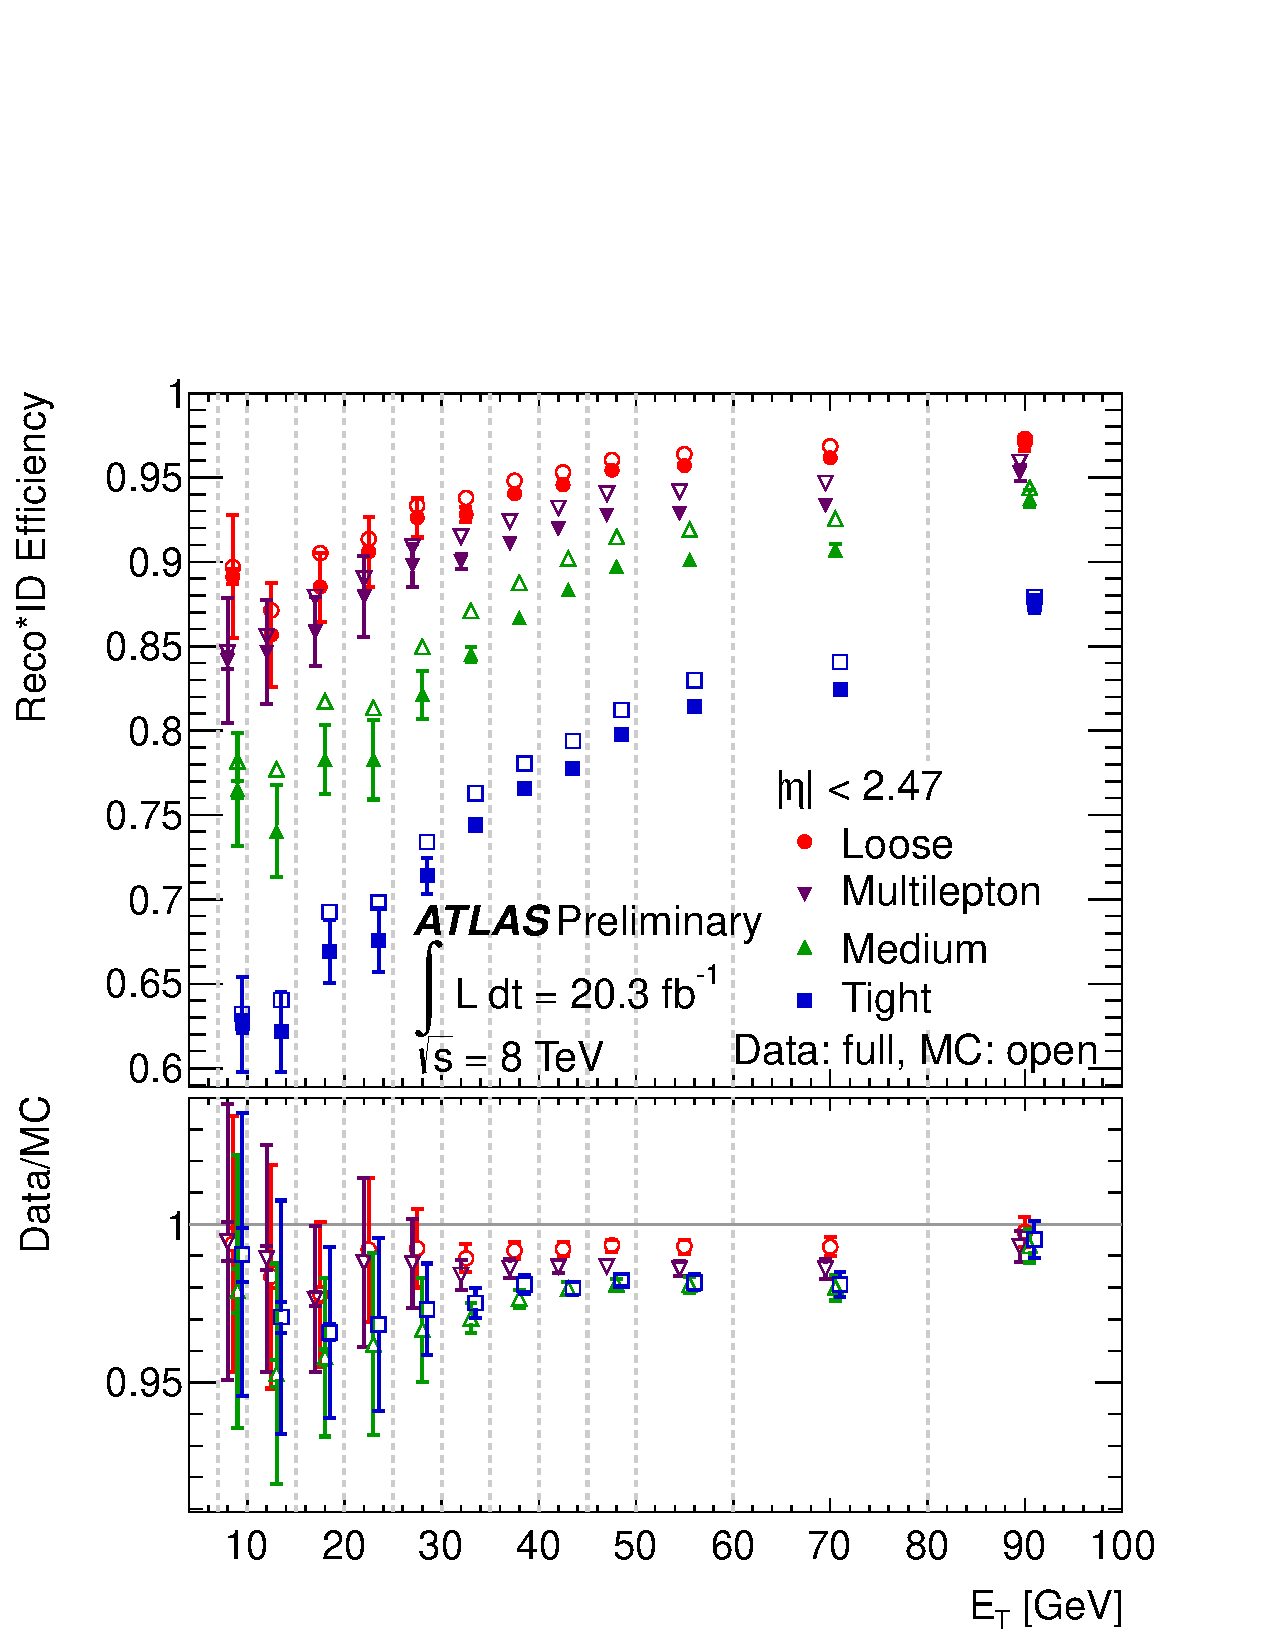
\includegraphics{figures/reconstruction/el_eff_idplusreco_ET}}
	}
	\hfill
	\subfloat[] {
		\resizebox{0.49\textwidth}{!}{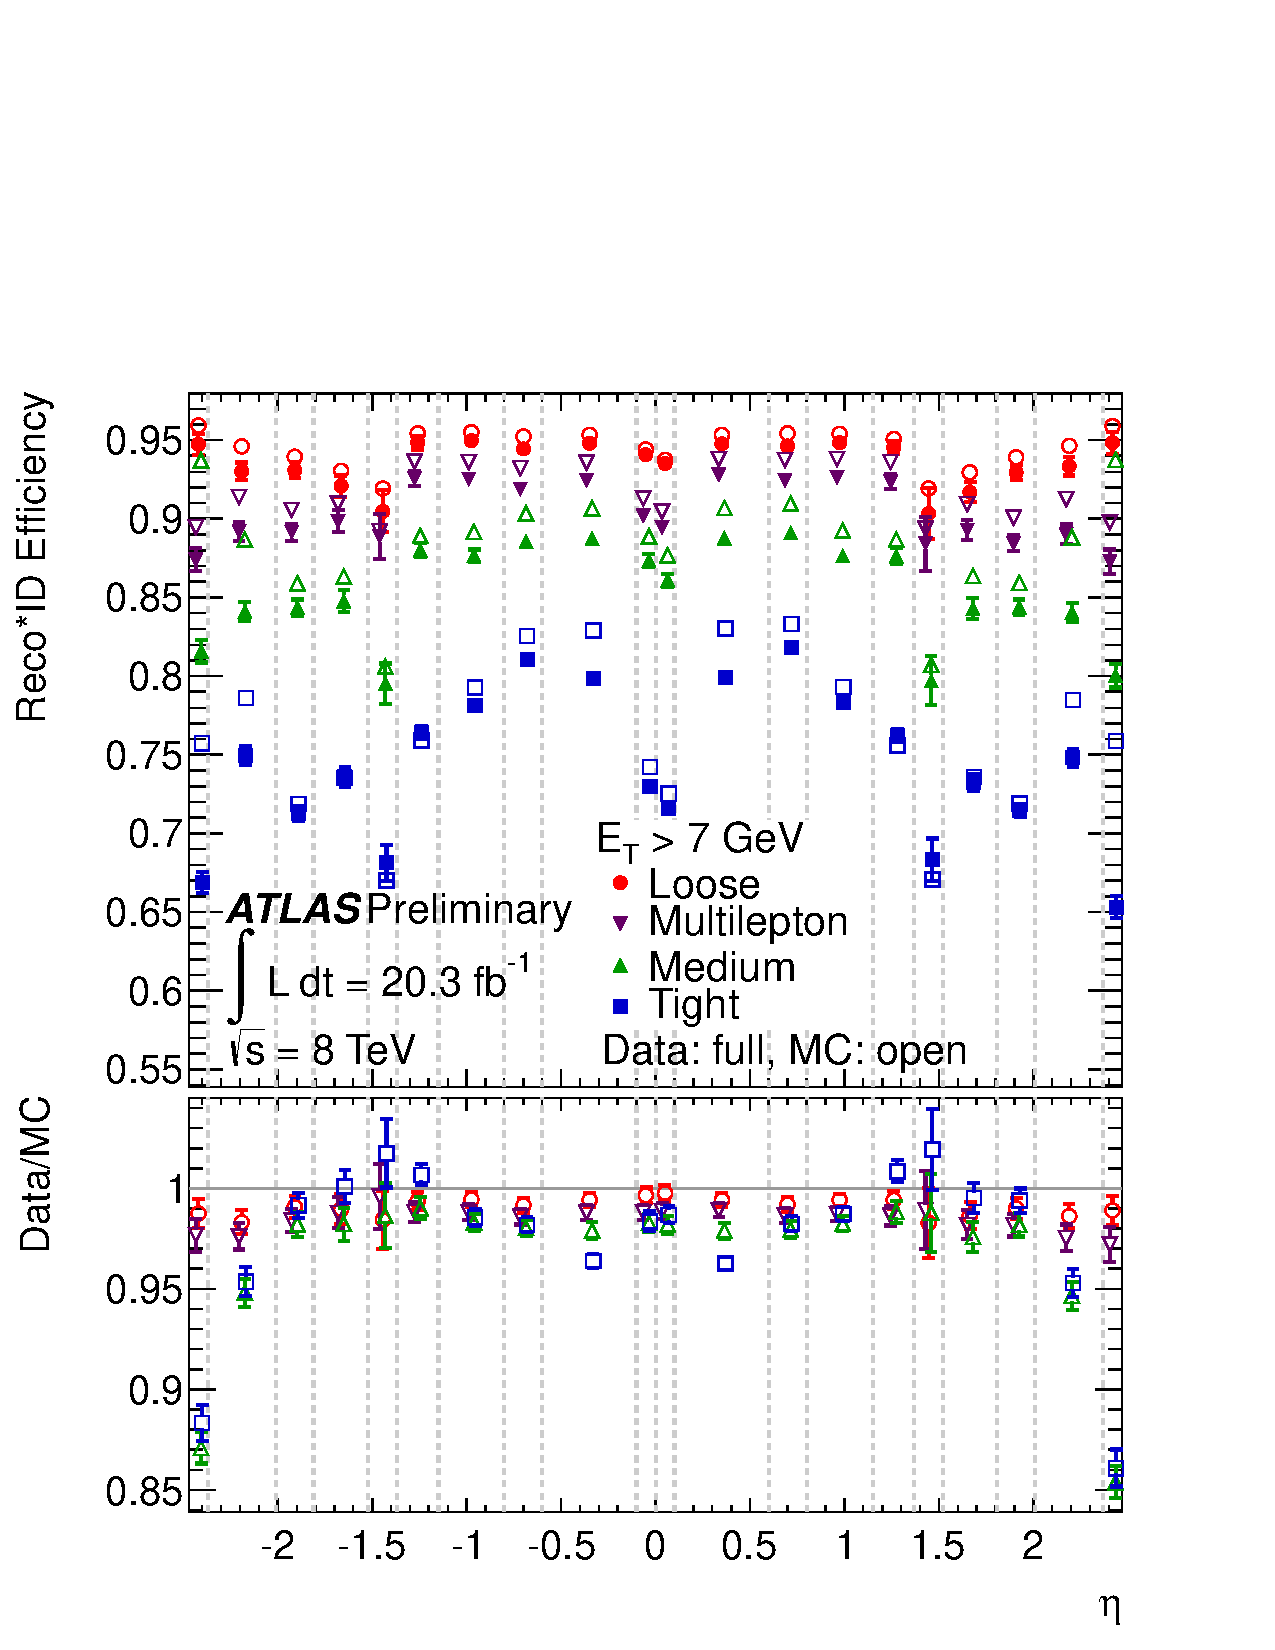
\includegraphics{figures/reconstruction/el_eff_idplusreco_eta}}
	}
	\caption{The combined reconstruction and identification efficiencies with respect to electrons detected as a cluster in the electromagnetic calorimeter, shown as a function of $\Et$ (left) and $\eta$ (right)~\cite{TheATLASCollaboration:2014vz}. The error bars show the statistical uncertainty (inner) and the statistical plus systematic uncertainty (outer). The ``multilepton'' identification cuts are optimized for low energy electrons in the $H\rightarrow ZZ^*\rightarrow 4\ell$ analysis, and are not used in this dissertation.}
	\label{fig:electron-id-efficiencies}
\end{figure}


\subsection{Energy and Momentum Measurement}\label{sec:reco-electron-energymomentum}
For electron candidates with at least four silicon hits, the energy of the electron is taken from the calorimeter measurement, while the trajectory is taken from the GSF track. Candidates with fewer than four silicon hits are not used in this dissertation. 

The energy measurement is calibrated using a multivariate algorithm trained on single-electron Monte Carlo (MC) simulation to determine the most probable electron energy. The method takes into account differences between data and simulation in the energy scales of each longitudinal layer and other detector effects not modeled in simulation. 

After the initial simulation-based calibration, the electron energy scale and resolution are determined using $Z\rightarrow ee$ events. Residual differences in the energy scale between data and simulation are parametrized as:

\begin{equation}
	E^{\mathrm{data}} = E^{\mathrm{simulation}} (1 + \alpha_i),
\end{equation}

where the $\alpha_i$ quantify the energy scale difference in bins of pseudorapidity. The difference in energy resolution is derived assuming that the $Z\rightarrow ee$ invariant mass distribution is well-modeled up to a Gaussian constant term, $c_i$: 

\begin{equation}
	\left(\frac{\sigma_E}{E}\right)^{\mathrm{data}} = \left(\frac{\sigma_E}{E}\right)^{\mathrm{simulation}} \oplus c_i,
\end{equation}

where $i$ again denotes bins in pseudorapidity. Histograms of the $Z\rightarrow ee$ invariant mass distribution in simulation are then produced for a range of $\alpha_i$ and $c_i$ values, and the optimal values are determined using a $\chi^2$ minimization with respect to data. The energy scale corrections are found to be $\alpha_i\sim -1\%$ in the barrel, $\sim1\%$--$2\%$ in the barrel/end-cap transition region, and up to $\sim-4\%$ in the end-caps. The resolution corrections are symmetrized about $\eta=0$, with values of $c_i\approx 0.8\%$ in the barrel, $\sim3.3\%$ in the barrel/end-cap transition region, and $\sim0.5\%$--$2.5\%$ in the end-caps. The energy resolution is shown as a function of $\ET$ in figure~\ref{fig:reco-el-EER}.

\begin{figure}[htbp]
	\centering
	\subfloat[ $|\eta|=0.2$] {
		\resizebox{0.45\textwidth}{!}{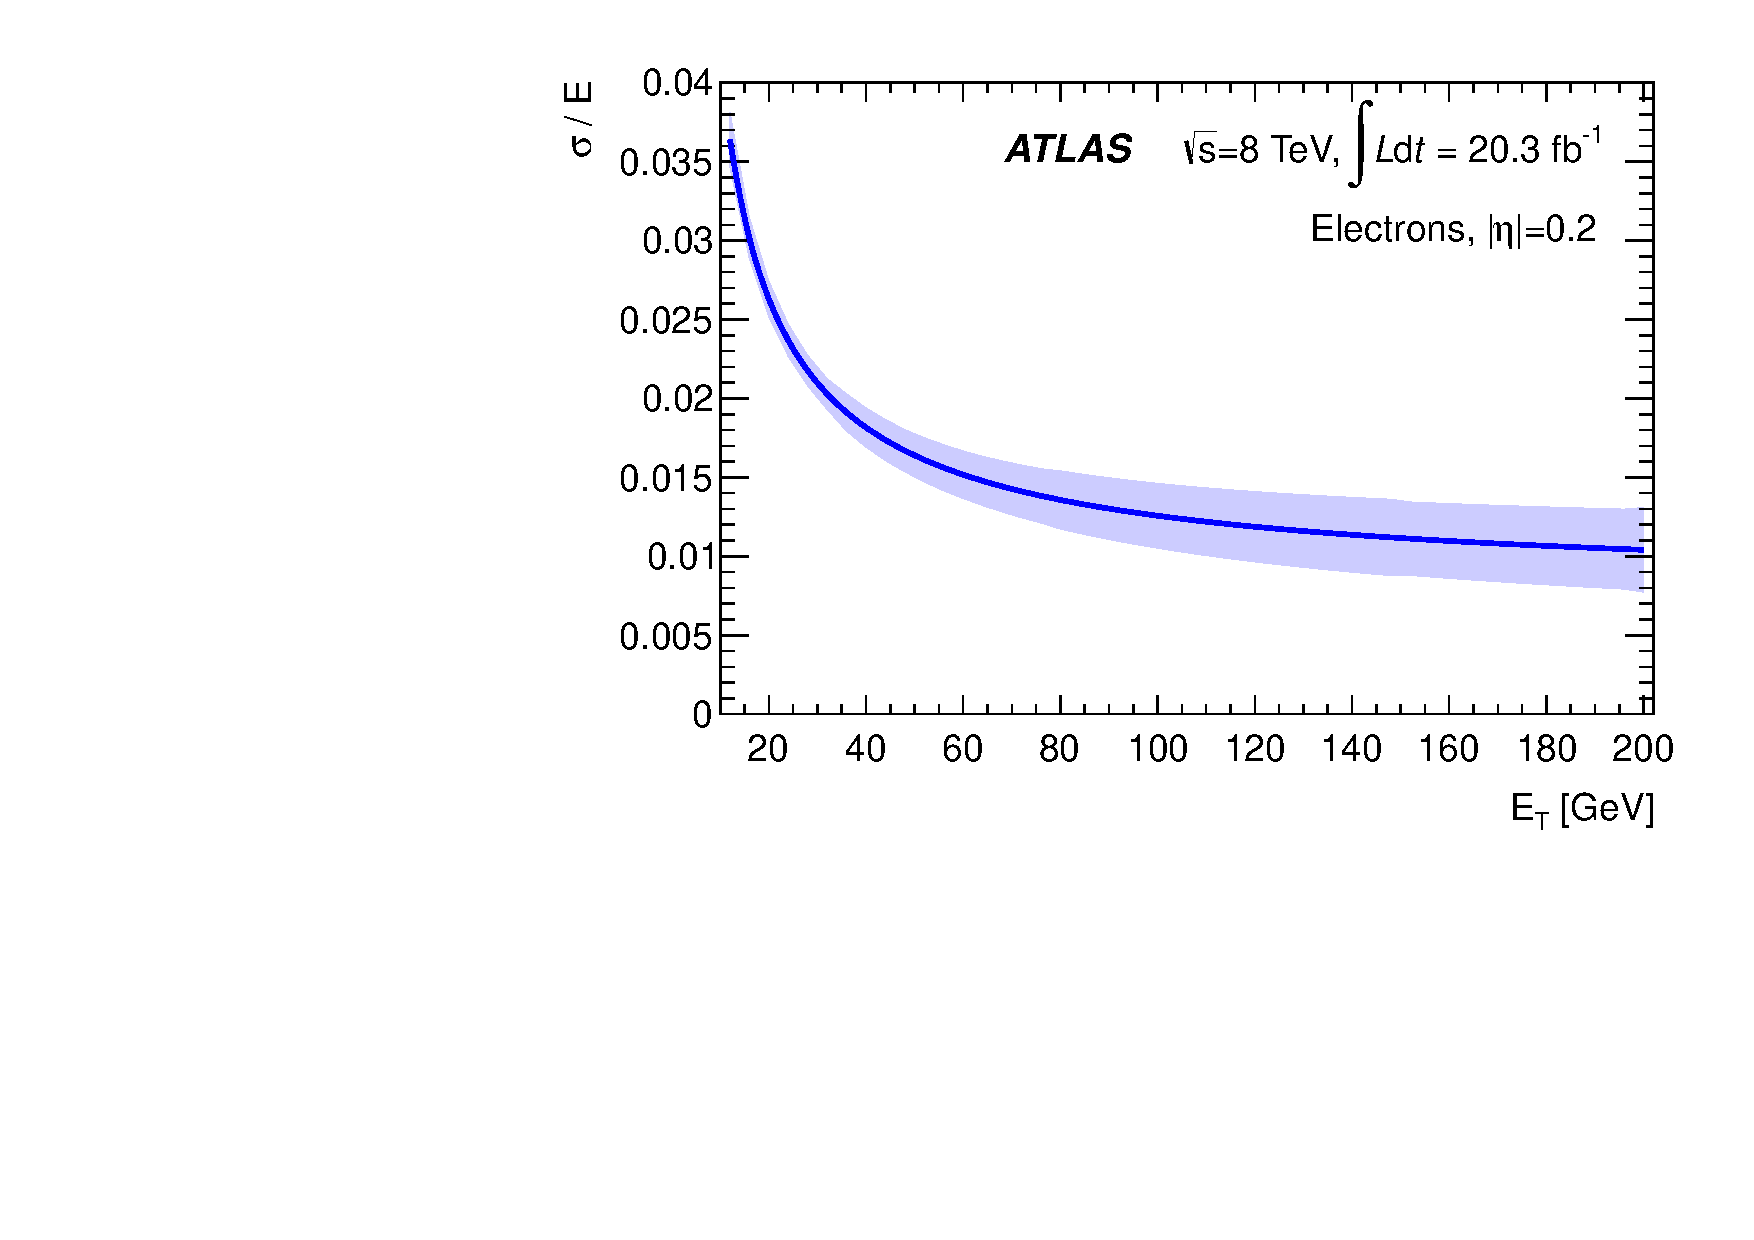
\includegraphics{figures/reconstruction/el_fig_35a}}
	}
	\hfill
	\subfloat[ $|\eta|=1.0$] {
		\resizebox{0.45\textwidth}{!}{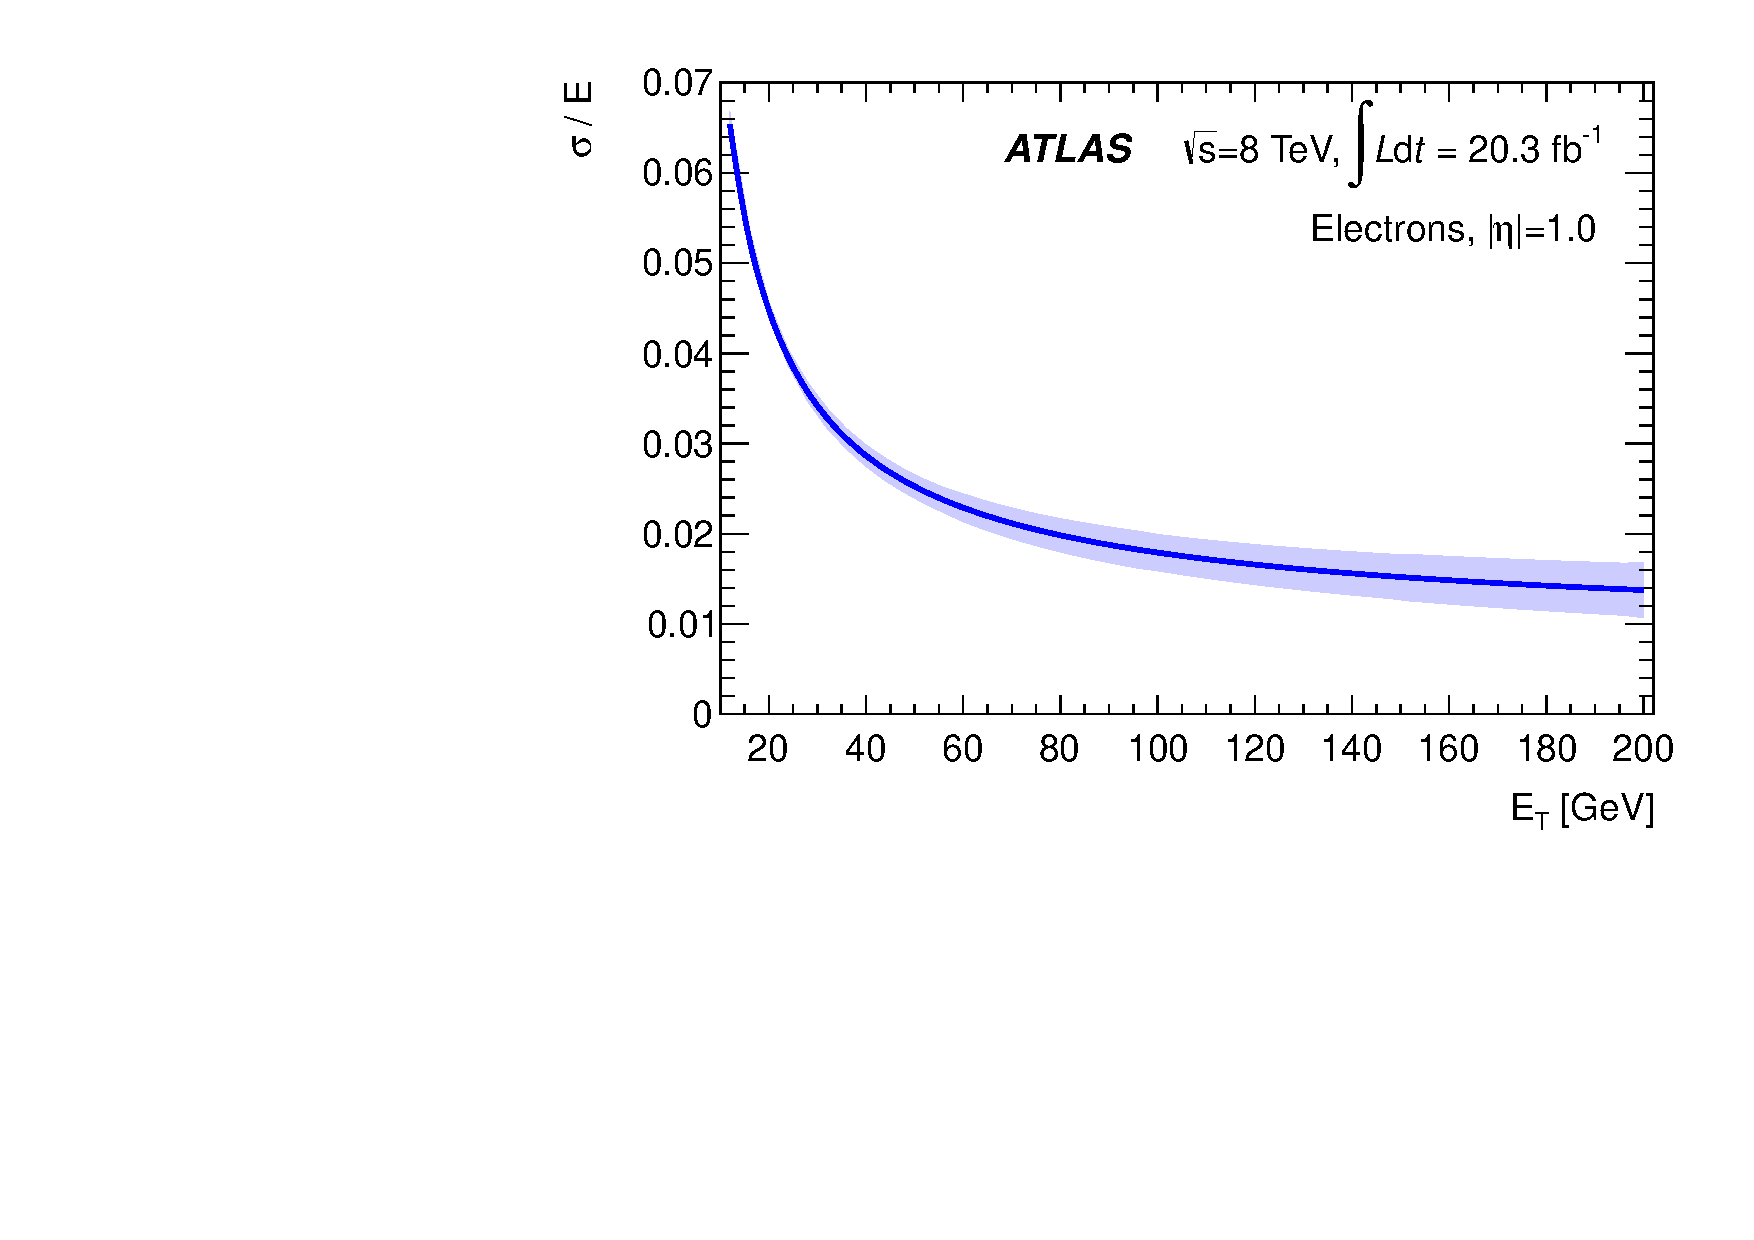
\includegraphics{figures/reconstruction/el_figaux_07a}}
	} \\
	\subfloat[ $|\eta|=1.7$] {
		\resizebox{0.45\textwidth}{!}{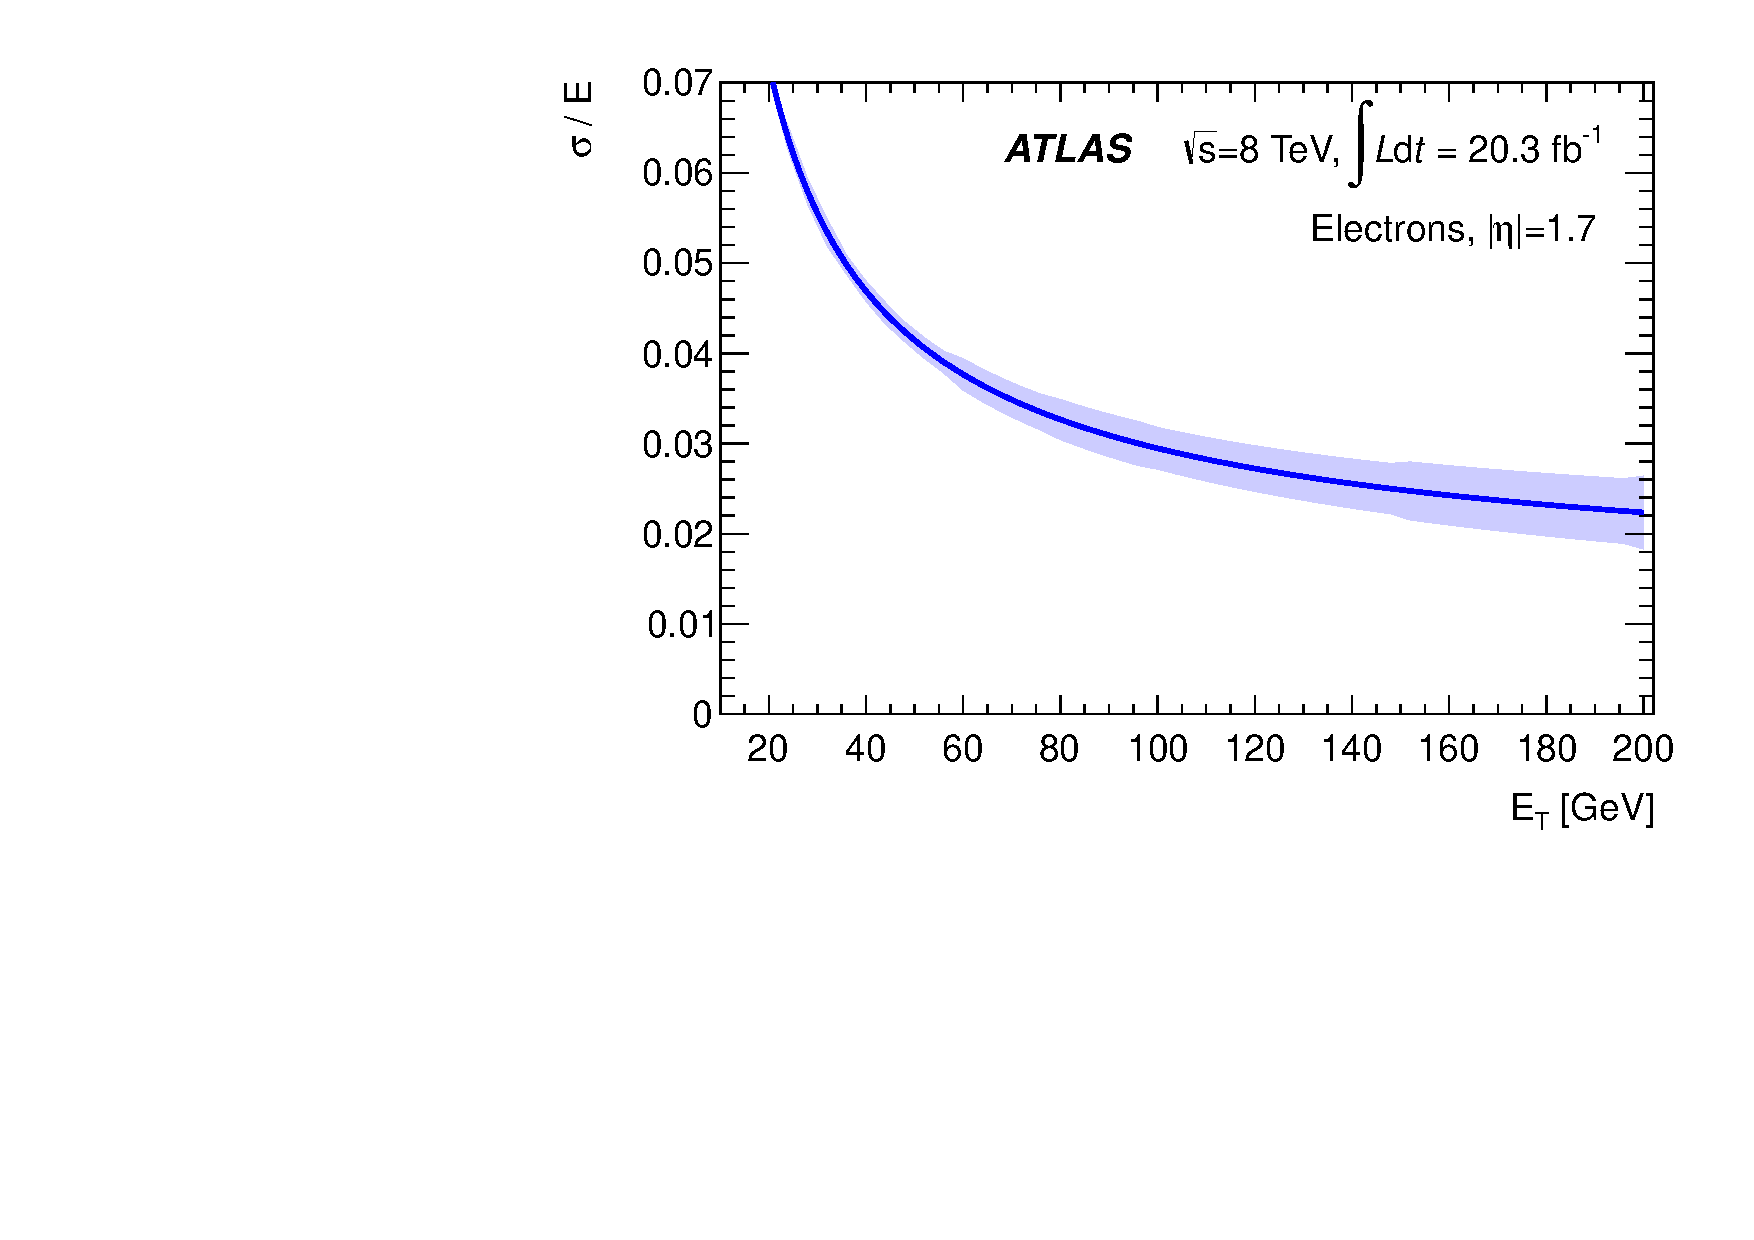
\includegraphics{figures/reconstruction/el_figaux_07c}}
	}
	\hfill
	\subfloat[ $|\eta|=2.1$] {
		\resizebox{0.45\textwidth}{!}{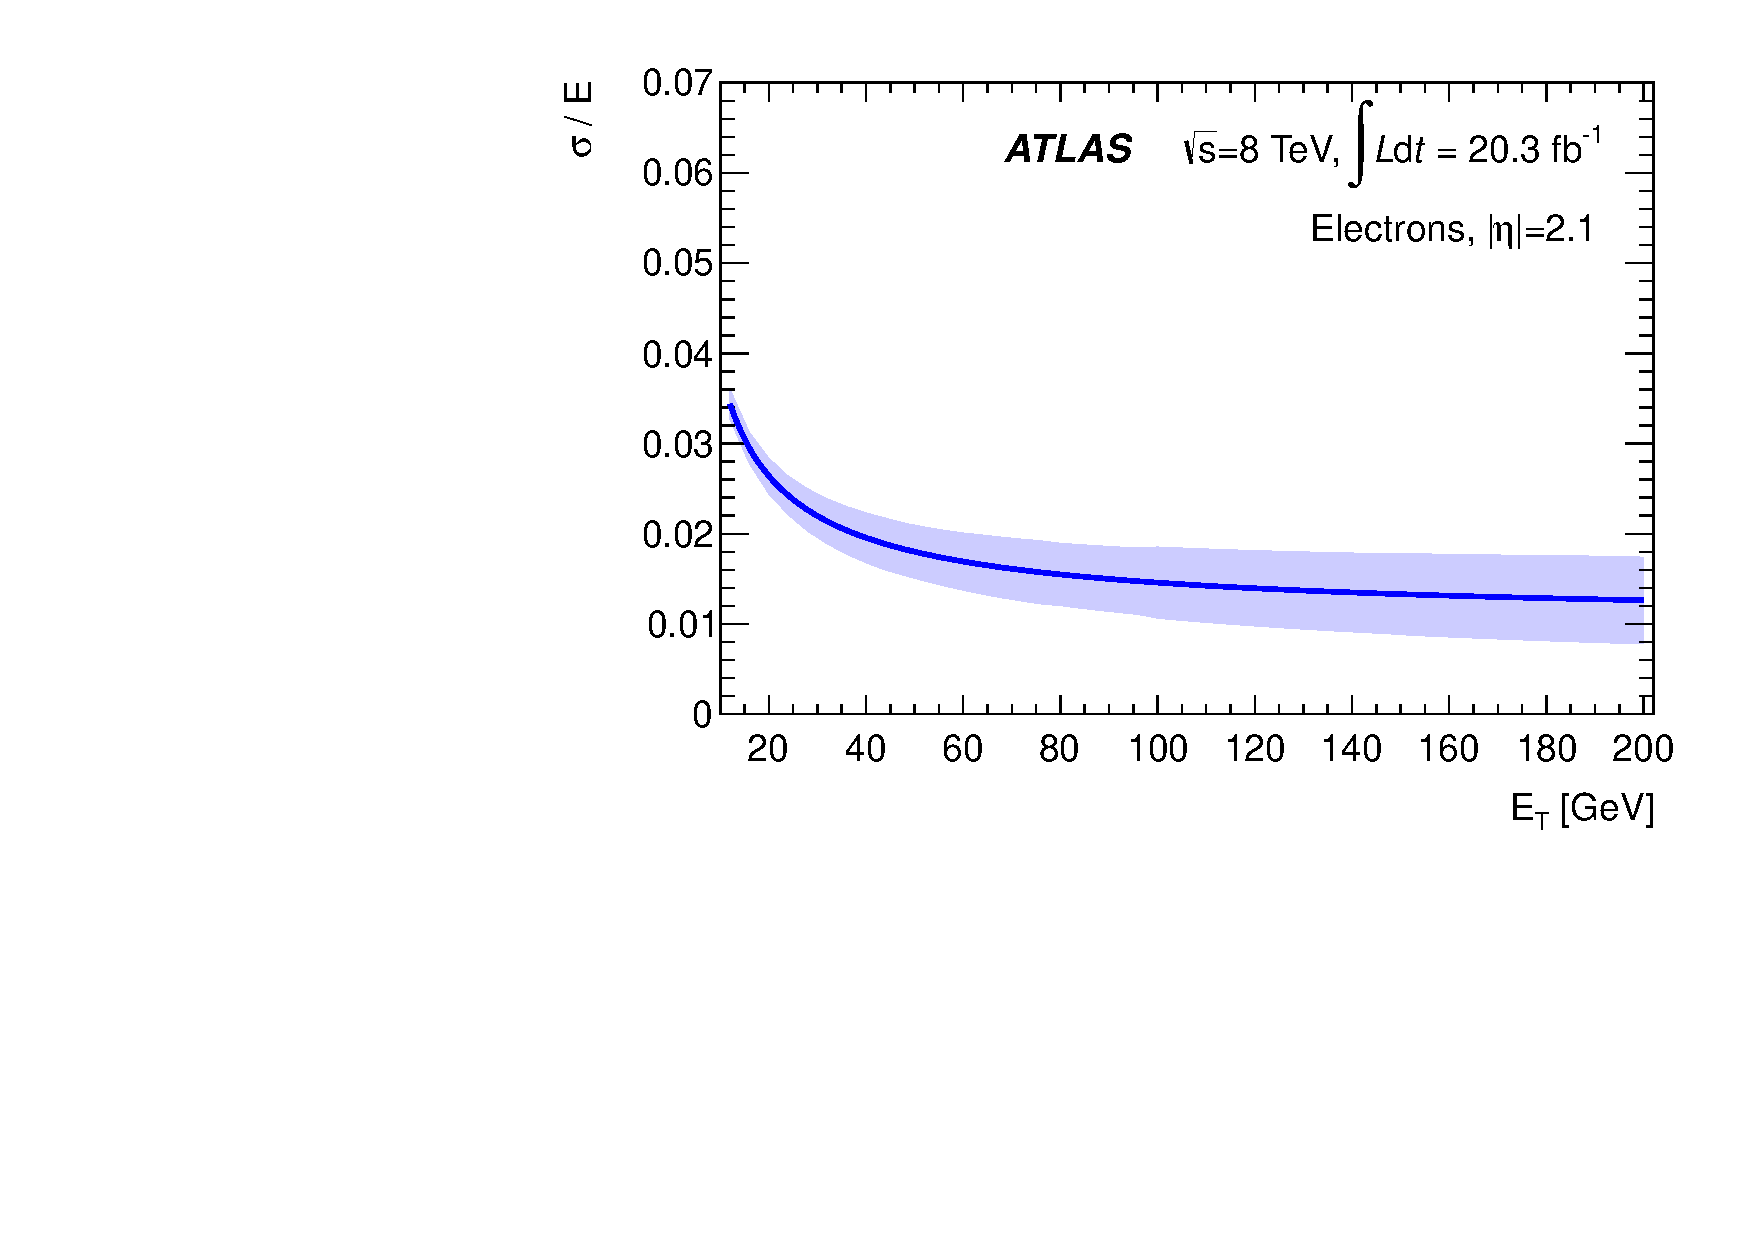
\includegraphics{figures/reconstruction/el_figaux_07e}}
	}
	\caption{Electron energy resolution as a function of $\ET$ for various values of $|\eta|$. The shaded band shows the uncertainty on the resolution~\cite{TheATLASCollaboration:2014gf}.}
	\label{fig:reco-el-EER}
\end{figure}


Sources of systematic uncertainty on the energy scale include the closure of the $Z\rightarrow ee$ method under injections of known energy scale variations, calorimeter gain and pedestal dependence, differences between data and simulation in the calibration of the calorimeter layers, and the modeling of material in front of and within the calorimeter. The total uncertainty ranges from $0.03\%$-$0.22$\% for $\Et=40 \GeV$ and $0.27\%$-$2.25$\% for $\Et = 200 \GeV$, with larger uncertainties in the pseudorapidity range $1.37<|\eta|<1.82$ corresponding to the transition region between the barrel and the end-cap. 

The systematic uncertainty on the energy resolution is less than $10\%$ for electrons with $\Et<50 \GeV$, and asymptotically approaches $\sim 40\%$ for high $\Et$. At low energies, the pileup contribution to the noise term, $b$, dominates the uncertainty; at higher energy, uncertainty is due to a mix of the sampling term, $a$, the pileup contribution to $b$, the modeling of material, and the intrinsic accuracy of the $Z\rightarrow ee$ method.


\section{Muons}\label{sec:event-reconstruction-muons}
Muons are reconstructed in several different ways, depending on the instrumentation available in the vicinity of the muon candidate~\cite{TheATLASCollaboration:2014bm}. The analyses described here use \emph{combined} (CB) muons, consisting of matched tracks reconstructed independently in the inner detector and the muon spectrometer (MS). The tracks in the MS are local track segments reconstructed within each MDT or CSC layer. The muon momentum is determined from a statistical combination of the two track's parameters and their corresponding covariance matrices. Combined muons have the highest purity, but suffer from a loss of acceptance near $\eta\sim 0$, where the muon spectrometer has gaps to accommodate services for the inner detector and calorimeters, and $1.1<\eta<1.3$, where some trajectories only pass through one muon station due to incomplete installation. The remaining categories are \emph{standalone} (SA) muons, consisting of a track only in the muon spectrometer; \emph{segment-tagged} (ST) muons, consisting of an inner detector track and one or more track segments in the MDT or CSC chambers; and \emph{calorimeter-tagged} (CaloTag) muons, consisting of an inner detector track matched to a calorimeter energy deposit consistent with the passage of a muon. These categories can recover efficiency in regions of the detector with less instrumentation at the cost of lower muon purity, but are not used in this dissertation. 

For all categories of muons, the inner detector track is required to have at least 1 pixel hit, at least 5 SCT hits, at most 2 pixel or SCT holes, and at least 9 TRT hits for $0.1<|\eta|<1.9$. Energy losses in the calorimeter due to ionization, bremsstrahlung, and electron pair production must also be taken into account. 

\subsection{Efficiency Measurements}\label{sec:reco-muon-efficiency}
The efficiency of the reconstructing CB muons is measured as:

\begin{equation}
	\epsilon(\mathrm{CB}) = \epsilon(\mathrm{CB}|\mathrm{ID}) \epsilon(\mathrm{ID}|\mathrm{MS}),
\end{equation}

where $\epsilon(\mathrm{CB}|\mathrm{ID})$ is the probability that a muon reconstructed as an inner detector track is also reconstructed as a CB muon, and $\epsilon(\mathrm{ID}|\mathrm{MS})\approx \epsilon(\mathrm{ID})$ is the probability that a muon with a track in the muon spectrometer, i.e. a CB or SA muon, is also reconstructed as an inner detector track. The latter approximation is made because $\epsilon(\mathrm{ID})$ is not directly accessible in data. 

The efficiencies are measured using tag-and-probe techniques similar to those described in section~\ref{sec:reco-electron-efficiency}, targeting $Z\rightarrow\mu\mu$ and $J/\Psi\rightarrow\mu\mu$ events. In this case, the tag muon is required to be a CB muon, and the probe muon is a CB or SA muon in the case of measuring $\epsilon(\mathrm{ID}|\mathrm{MS})$, and a CaloTag muon for the measurement of $\epsilon(\mathrm{CB}|\mathrm{ID})$. The efficiencies for all types of muon are shown in figure~\ref{fig:reco-muon-efficiency}. CB muons have an efficiency of greater than $97\%$ in most of the pseudorapidity range, except for significant inefficiencies due to gaps in the muon spectrometer in the ranges $|\eta|<0.1$ and $1.1<\eta<1.3$. The measured efficiencies in data and simulation agree to within $\sim2\%$, and the ratios in each pseudorapidity bin are used as scale factors to correct the efficiency in simulation. The systematic uncertainty on the scale factors is below $0.2\%$ for most of the pseudorapidity range, rising to $\sim 0.3\%$ near $|\eta|\sim 2.5$ and $\sim0.7\%$ near $|\eta|\sim 0$. 

\begin{figure}[htbp]
	\centering
	\subfloat[] {
		\resizebox{0.45\textwidth}{!}{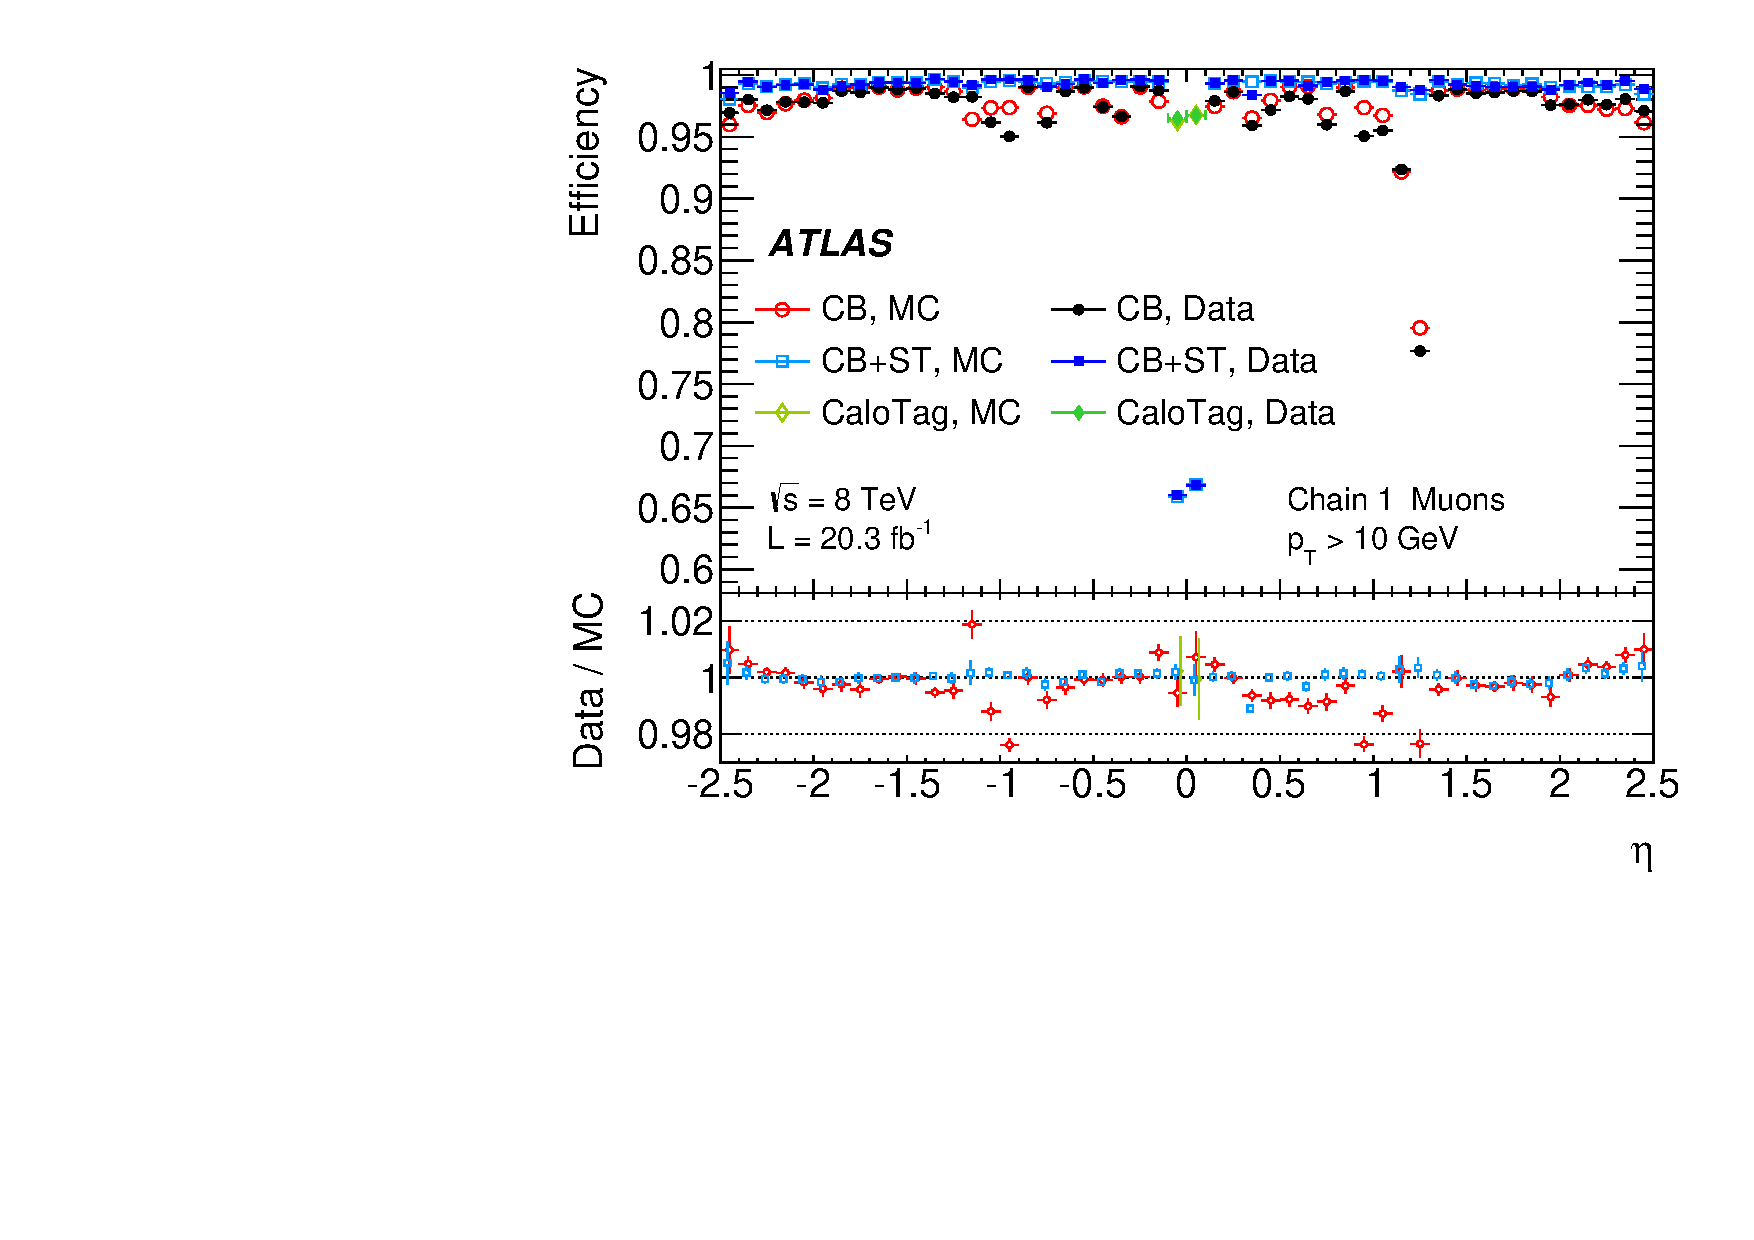
\includegraphics{figures/reconstruction/mu_fig_03}}
	}
	\hfill
	\subfloat[] {
		\resizebox{0.45\textwidth}{!}{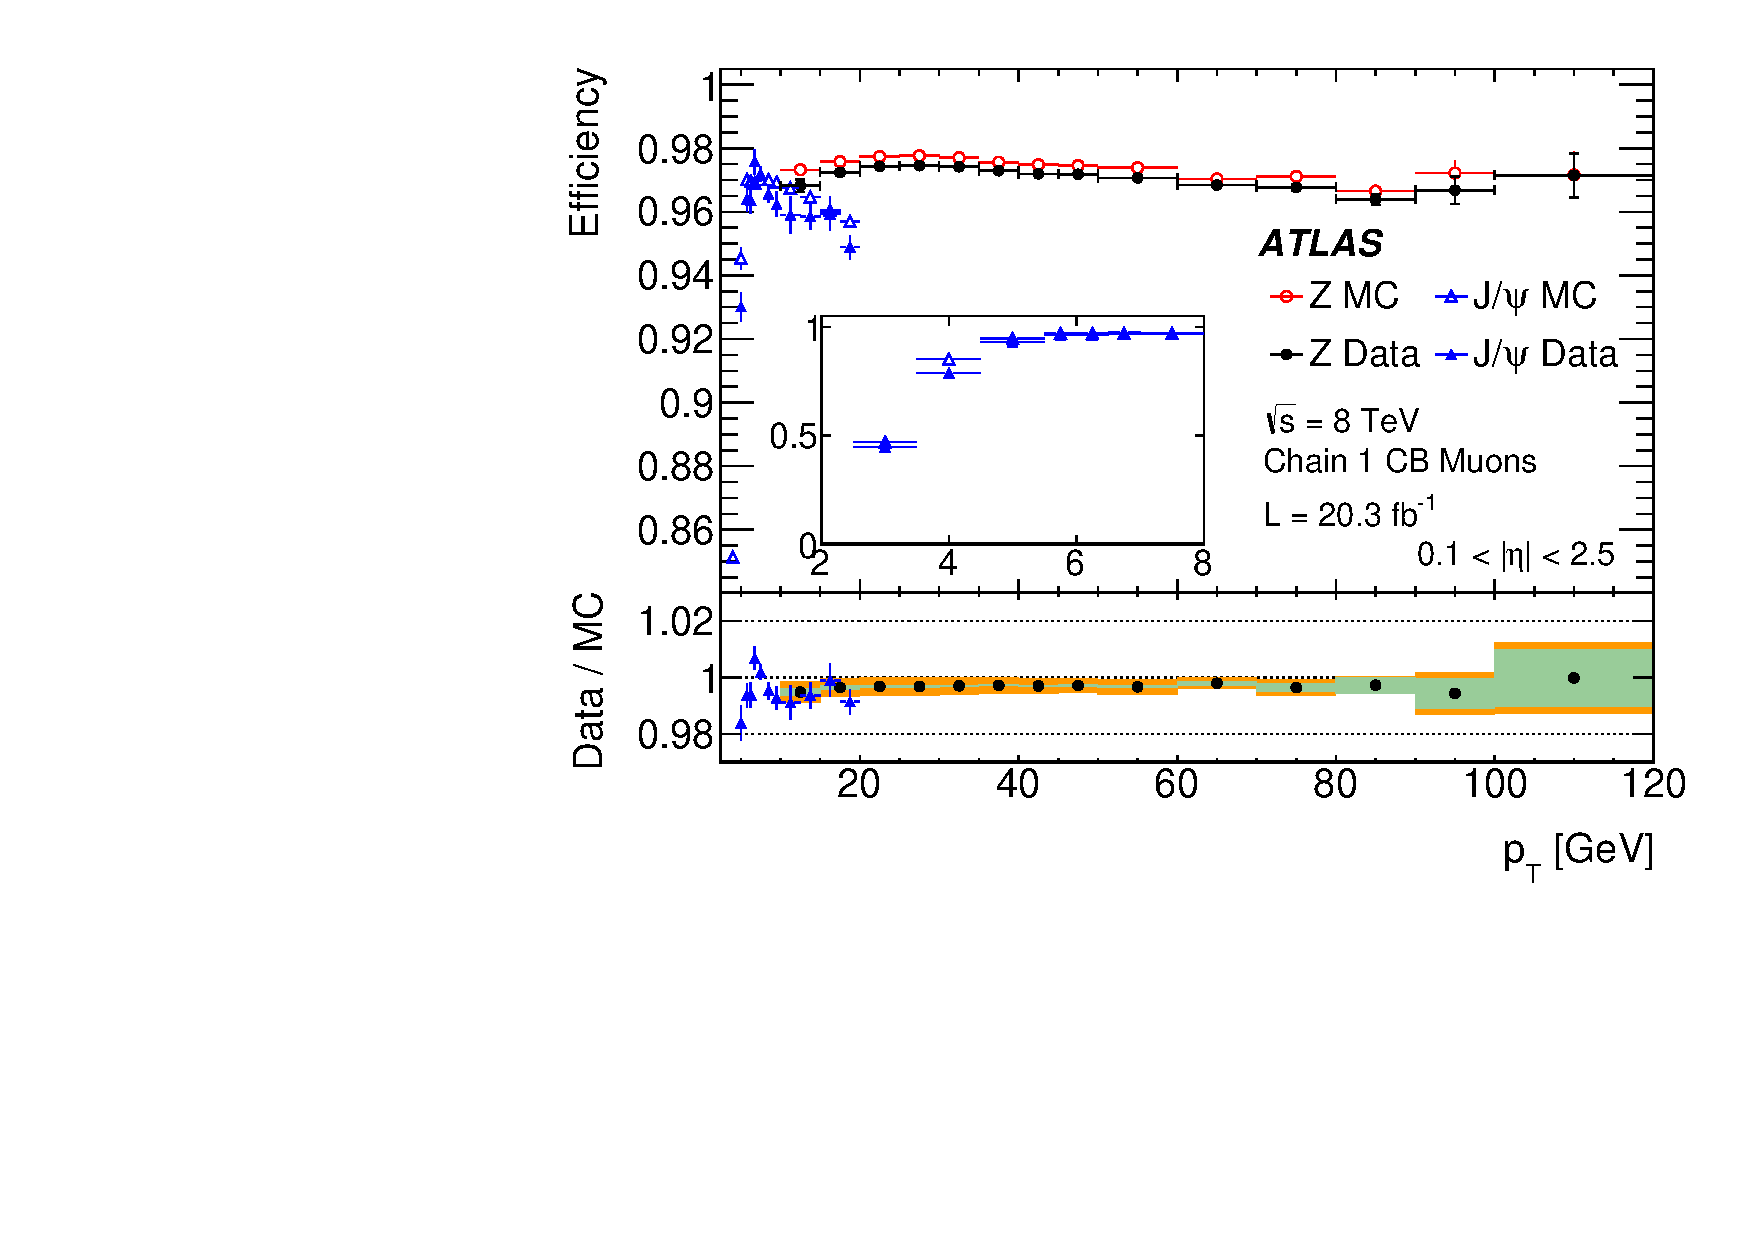
\includegraphics{figures/reconstruction/mu_fig_05a}}
	}
	\caption{Muon reconstruction efficiencies as a function of $\eta$ for muons with $\pt>10 \GeV$ (left), and as a function of $\pt$ for muons with $0.1<|\eta|<2.5$ (right)~\cite{TheATLASCollaboration:2014bm}. The uncertainty bars on the points indicate statistical uncertainties. The bottom plots show the ratio between the measured and simulated efficiencies, with the combination of statistical and systematic uncertainties indicated by the uncertainty bars.}
	\label{fig:reco-muon-efficiency}
\end{figure}


\subsection{Energy Scale and Resolution}\label{sec:reco-muon-energymomentum}
The muon momenta in simulation are scaled and smeared to match the momentum scale and resolution in data. The corrections are derived in bins of $\eta$ and $\phi$, with boundaries chosen to minimize the variation of the correction in each bin, and are applied separately to the transverse momenta measured by the inner detector (ID) and the muon spectrometer (MS). Specifically, the correction is implemented as:

\begin{equation}
	\pt^{\mathrm{Cor,Det}} = \frac{\pt^{\mathrm{MC,Det}} + \sum_{n=0}^1 s_n^{\mathrm{Det}(\eta,\phi)(\pt^{\mathrm{MC,Det}})^n}}{1+\sum_{m=0}^2 \Delta r_m^{\mathrm{Det}}(\eta,\phi)(\pt^{\mathrm{MC,Det}})^{m-1}g_m},
\end{equation}

where Det=ID or MS, the $\Delta r_m^{\mathrm{Det}}(\eta,\phi)$ parametrize the momentum resolution smearing, the $s_n^{\mathrm{Det}}(\eta,\phi)$ parametrize the scale corrections, and the $g_m$ are normally-distributed random variable with mean 0 and width 1\footnote{Note that this equation does not apply to cases where the resolution is data is better than that in simulation. In these cases, the resolution difference is included in the positive ID and MS variations, and the effect of the positive variation on the physical observables is symmetrized about the nominal value.}. The constant scale correction term, $s_0^{\mathrm{MS}}$, accounts for the difference between data and simulation in the energy lost by muons before reaching the muon spectrometer. $s_0^{\mathrm{ID}}$ is set to zero due to the negligible energy loss before the inner detector. The linear terms, $s_1^{\mathrm{ID,MS}}$, models discrepancies between data and simulation in the magnetic field integral and the radial dimension of the detector. The resolution corrections $\Delta r_m^{\mathrm{Det}}$ represent deviations from the resolution in data, which is parametrized empirically as:

\begin{equation}
	\frac{\sigma(\pt)}{\pt} = \frac{r_0}{\pt} \oplus r_1 \oplus r_2\cdot\pt,
\end{equation}

where the $r_0$ term describes energy lost by muons as they traverse the material of the detector, the $r_1$ term describes multiple scattering, magnetic field inhomogeneities, and local radial displacements, and the $r_2$ term describes intrinsic resolution effects due to the spatial resolution of the hit measurements and residual misalignment. 

The corrections are derived from $J/\Psi\rightarrow\mu\mu$, $\Upsilon\rightarrow\mu\mu$, and $Z\rightarrow\mu\mu$ events using a template maximum likelihood fit, similar to that described in section~\ref{sec:reco-electron-energymomentum}. The effect of the corrections on the invariant mass distribution of $Z\rightarrow\mu\mu$ events is shown in figure~\ref{fig:reco-muon-momentum-corrections}, along with the total systematic uncertainty. The muon resolution as measured in $Z$, $\Upsilon$, and $J/\Psi$ events is shown in figure~\ref{fig:reco-muon-resolution}.

\begin{figure}[htbp]
	\centering
	\resizebox{0.6\textwidth}{!}{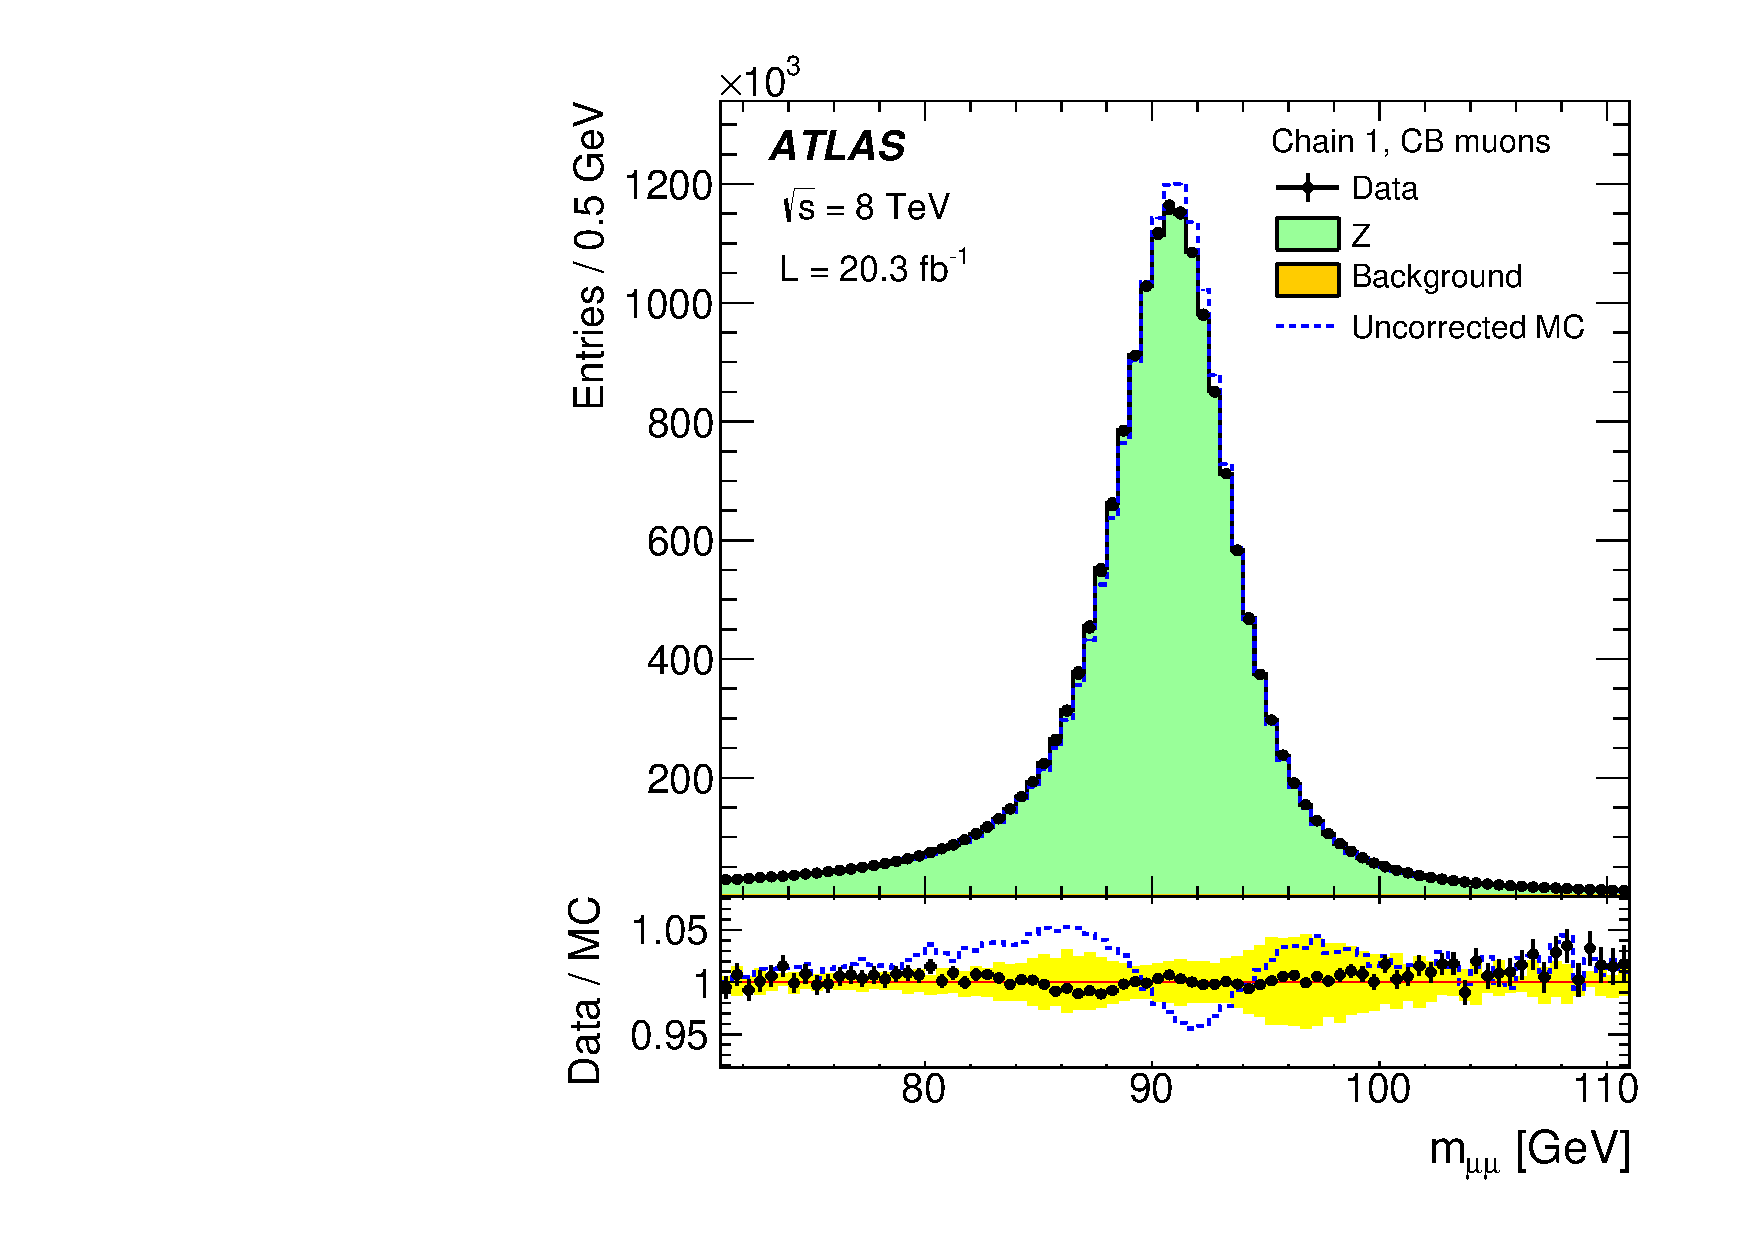
\includegraphics{figures/reconstruction/mu_fig_10c}}
	\caption{Dimuon invariant mass distribution of $Z\rightarrow\mu\mu$ events, using CB muons~\cite{TheATLASCollaboration:2014bm}. The top panel shows the invariant mass distribution for data (black points), expected $Z\rightarrow\mu\mu$ signal from MC simulation (green), and expected background from MC simulation (yellow). The muon momentum corrections are applied to the MC simulation, and the total MC prediction is normalized to the data. The dashed histogram shows the background plus signal without muon momentum corrections. The bottom panel shows the ratio of the data to the normalized MC prediction, with the systematic uncertainty on the momentum corrections shown in the yellow band.}
	\label{fig:reco-muon-momentum-corrections}
\end{figure}

\begin{figure}[htbp]
	\centering
	\subfloat[ $|\eta|<1$] {
		\resizebox{0.3\textwidth}{!}{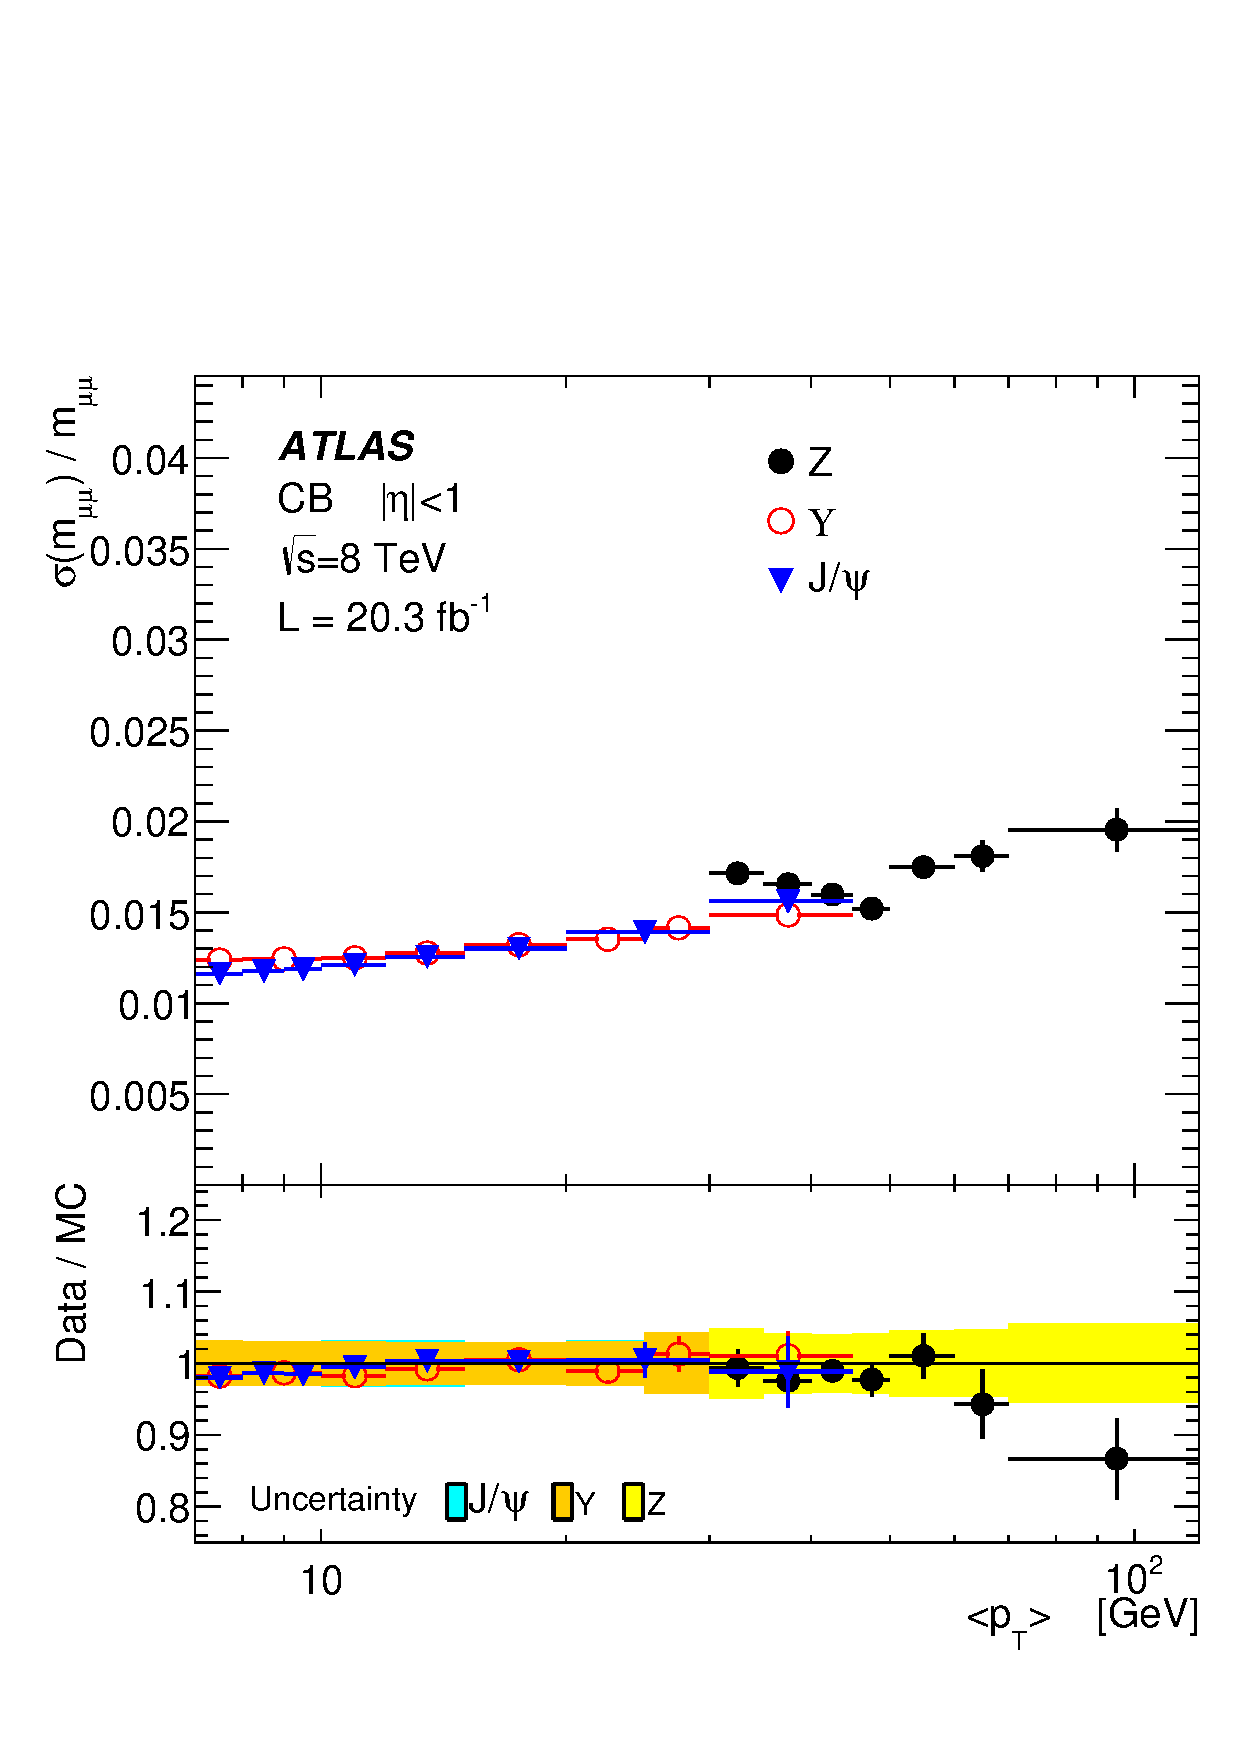
\includegraphics{figures/reconstruction/mu_fig_14a}}
	}
	\hfill
	\subfloat[ $1<|\eta|<2$] {
		\resizebox{0.3\textwidth}{!}{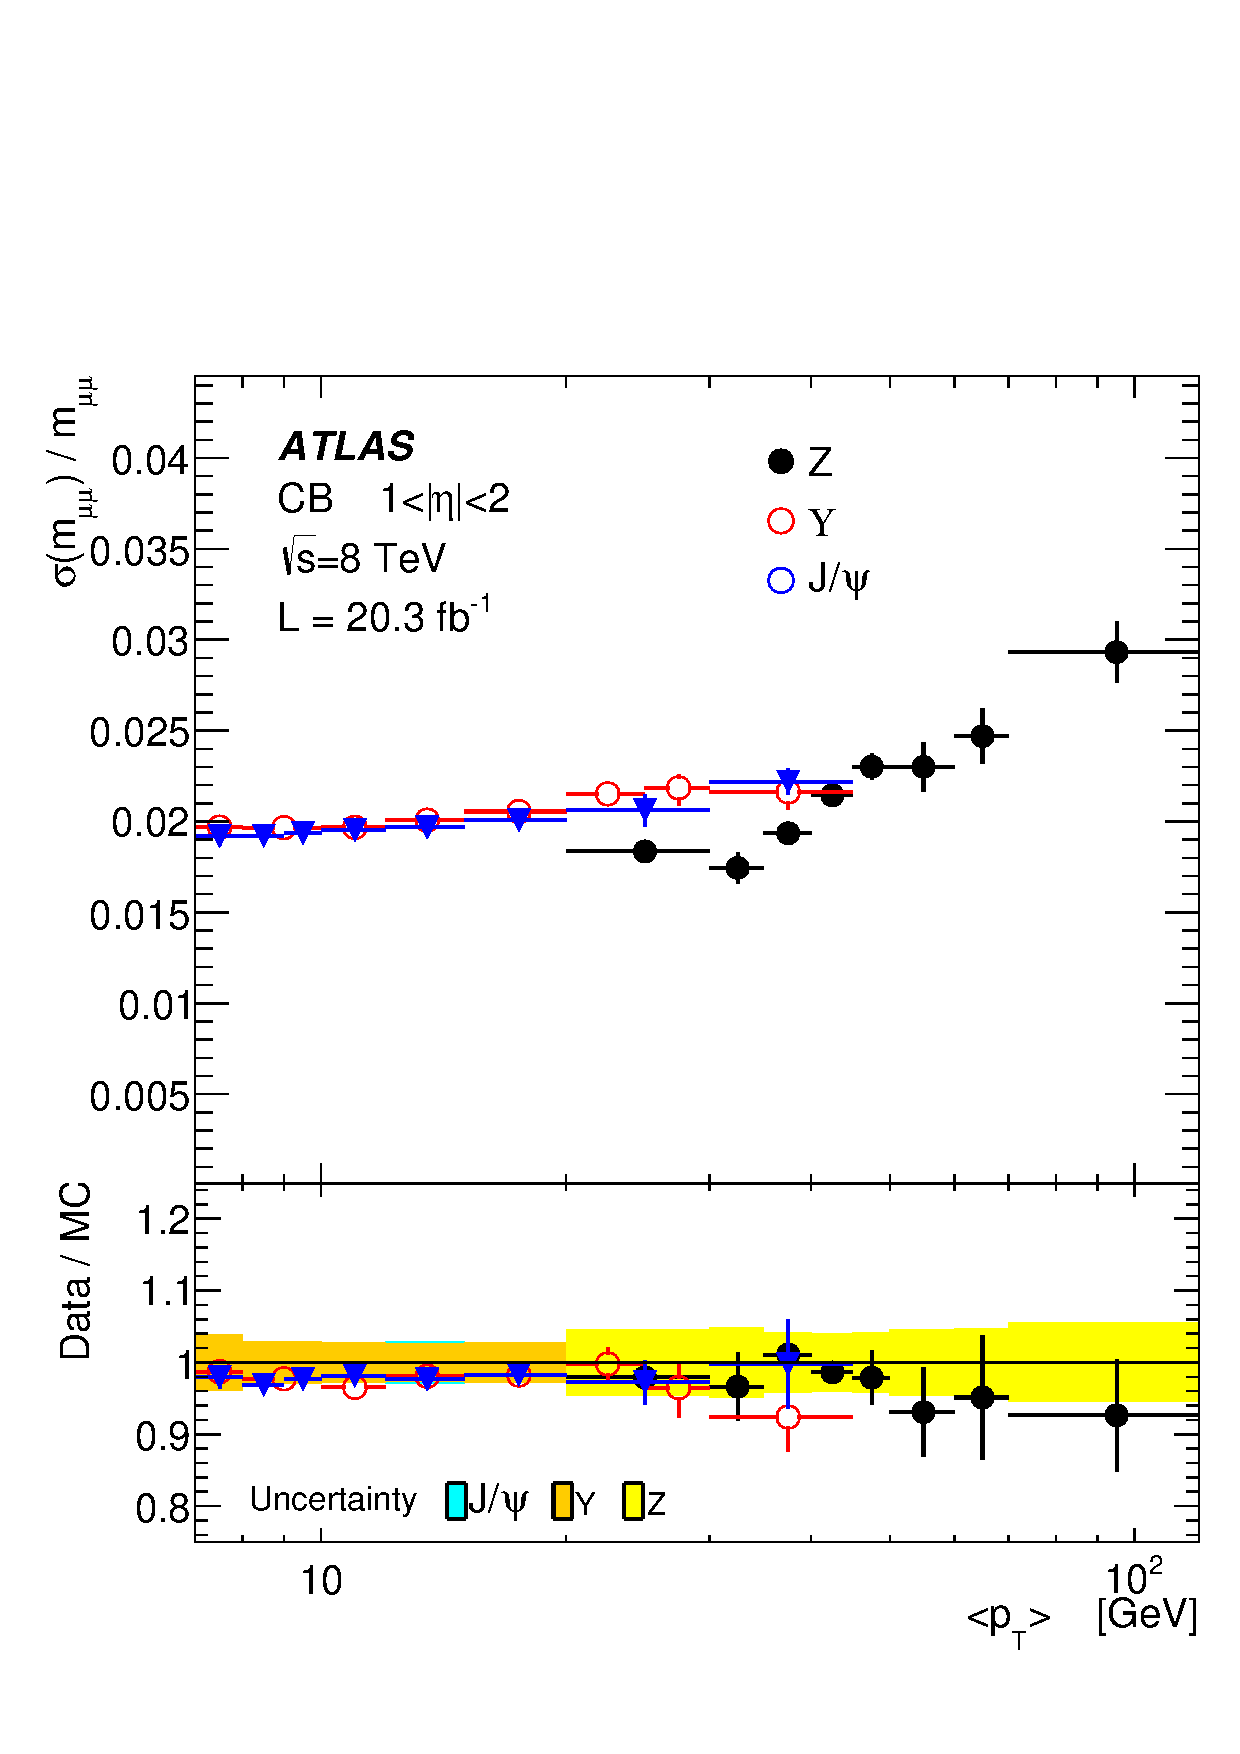
\includegraphics{figures/reconstruction/mu_fig_14b}}
	}
	\hfill
	\subfloat[ $|\eta|>2$] {
		\resizebox{0.3\textwidth}{!}{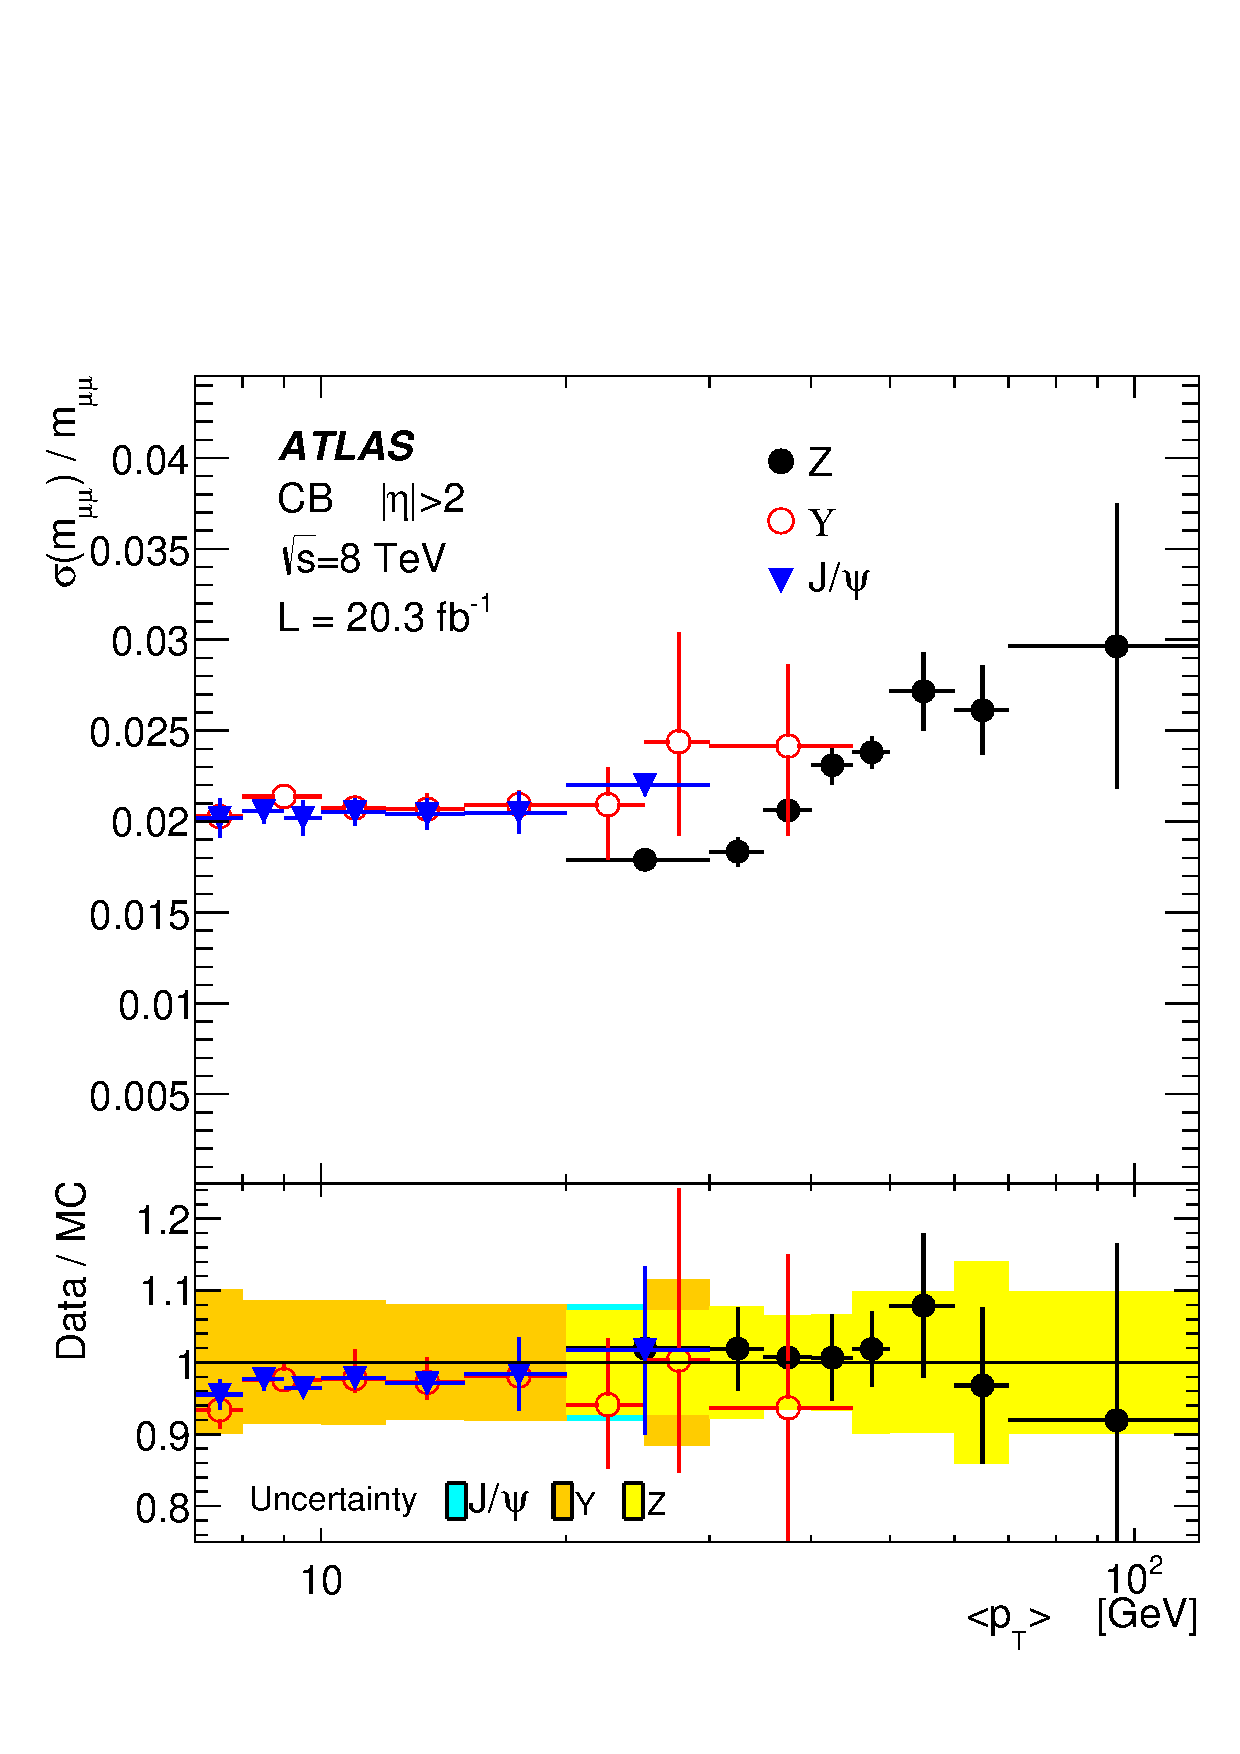
\includegraphics{figures/reconstruction/mu_fig_14c}}
	}
	\caption{Dimuon invariant mass resolution for combined muons as a function of the average muon $\pt$ in three pseudorapidity regions. The resolution is determined from $J/\Psi\rightarrow\mu\mu$, $\Upsilon\rightarrow\mu\mu$, and $Z\rightarrow\mu\mu$ events. Both muons are required to be in the same pseudorapidity region. The $J/\Psi$ and $\Upsilon$ data are plotted as a function of $\bar{\pt}=\frac{p_{\mathrm{T}1}+p_{\mathrm{T}2}}{2}$, while $Z$ data are plotted as a function of $\pt^*=m_{Z}\sqrt{\frac{\sin\theta_1\sin\theta_2}{2(1-\cos\alpha_{12})}}$, where $\theta_{1,2}$ are the polar angles of the two muons and $\alpha_{12}$ is the angle between the two muons, which removes the correlation between $m_{\mu\mu}$ and $\bar{\pt}$.  The lower panels show the ratio between data and the corrected MC, with bands representing the uncertainty on the MC corrections for the three calibration samples.}
	\label{fig:reco-muon-resolution}
\end{figure}


\section{$\tau$ Leptons}\label{sec:event-reconstruction-taus}
The signature of $\tau$ leptons is significantly more complex than electrons and muons due to the fact that they decay to a diverse set of final states. Tau leptons have a proper decay length of $87 \micron$, and therefore typically decay before reaching the active layers of the detector. The leading decay modes are shown in table~\ref{table:reco-tau-decays}. The branching fractions to $e\overline{\nu}_e\nu_{\tau}$ or $\mu\overline{\nu}_{\mu}\nu_{\tau}$ are 17.83\% and 17.41\%, respectively. The remaining $64.8\%$ of decays are to hadrons plus a neutrino. The hadronic decay modes contain one charged pion in $72\%$ of the decays, and three charged pions in $22\%$ of the decays; the majority of the remainder contain one or more kaons. The hadronic decay modes also frequently contain neutral pions, with $78\%$ containing at least one neutral pion. 


\begin{table}[htbp]
	\centering
	\begin{tabular}{|l|c|}
		\hline
		Decay & Branching Fraction [\%] \\
		\hline
		$e^- \overline{\nu}_e \nu_{\tau}$ & $17.83 \pm 0.04$ \\
		\hline
		$\mu^- \overline{\nu}_{\mu} \nu_{\tau}$ & $17.41 \pm 0.04$ \\
		\hline
		$\pi^- \nu_{\tau}$ & $10.83 \pm 0.06$ \\
		\hline
		$\pi^- \pi^0 \nu_{\tau}$ & $25.52 \pm 0.09$ \\
		\hline
		$\pi^- \pi^0\pi^0\nu_{\tau}$ & $ 9.30 \pm 0.11$ \\
		\hline
		$\pi^-\pi^+\pi^-\nu_{\tau}$ & $9.31 \pm 0.06$ \\
		\hline
		$\pi^-\pi^+\pi^-\pi^0\nu_{\tau}$ & $4.62 \pm 0.06$ \\
		\hline
	\end{tabular}
	\caption{Leading branching fractions of the $\tau$ lepton to final states with leptons or pions. Most of the remaining decays are to final states with kaons. From~\cite{pdg}.}
	\label{table:reco-tau-decays}
\end{table}

In this dissertation, no effort is made to identify or reconstruct leptonic $\tau$ decays ($\tau_{\mathrm{lep}}$), regarding them only as electrons or muons plus missing transverse energy (see section~\ref{sec:reco-met}). Hadronic $\tau$ decays ($\tau_{\mathrm{had}}$) are identified using their visible decay products, namely the neutral and charged hadrons, which are collectively called $\tau_{\mathrm{had-vis}}$. The signature consists of a narrow jet with one or three tracks, called one-prong or three-prong decays, respectively. Up to two $\pi^0\rightarrow\gamma\gamma$ decays are also included. The reconstruction and identification proceeds as follows~\cite{TheATLASCollaboration:2014tga}:

\begin{itemize}
	\item Jets are reconstructed using the anti-$k_t$ algorithm with a distance parameter of $R=0.4$, built from TopoClusters calibrated with a local hadronic calibration. Jets with $\pt>10 \GeV$ and $|\eta|<2.5$ are used as seeds for $\tau$ lepton candidates.

	\item For each jet seed, the $\tau$ vertex is chosen to be the primary vertex with the greatest $\sum \pt$ of tracks in a cone of radius $\Delta R=0.2$ around the jet seed. This vertex defines the $\tau_{\mathrm{had-vis}}$ direction, i.e. is used to determine the $\eta$ and $\phi$ of the $\tau$ candidate. 

	\item $\pi^0$ candidates, consisting of a pair clusters within $\Delta R<0.2$ of the $\tau$ candidate, are identified using a multivariate boosted decision tree (BDT) algorithm. The algorithm identifies up to two $\pi^0$s.

	\item BDT-based identification algorithms are used to discriminate hadronic $\tau$ decays from the backgrounds, primarily due to jets with low track multiplicity. The BDTs use many input variables describing the energy cluster, the spatial arrangement and energy of the tracks, and the neutral pions. Separate BDTs are trained for one-prong and three-prong $\tau$ decays, using simulated $Z\rightarrow\tau\tau$, $W\rightarrow \tau\nu$, and $Z'\rightarrow\tau\tau$ decays for signal and collision data samples for the background. Three working points with different identification efficiencies are defined: \texttt{BDT-loose}, \texttt{BDT-medium}, and \texttt{BDT-tight}. The performance of the identification algorithms is shown in figure~\ref{fig:reco-tau-efficiency}. The correction factors applied to simulated samples to equalize the efficiencies in simulation and real data are shown in figure~\ref{fig:reco-tau-efficiency-scale-factors}. The correction factors are derived by measuring the efficiencies in data and simulation, using a tag-and-probe method targeting $Z\rightarrow\tau_{\mathrm{lep}}\tau_{\mathrm{had}}$ events. For the \texttt{BDTTight} working point, the corrections range from $94\%$-$96\%$, and carry uncertainties between $2.0\%$-$2.2\%$. 

	\item An additional BDT-based algorithm rejects one-prong $\tau$ candidates consistent with an electron. The most powerful discriminating variables are the ratio of high- to low-threshold TRT hits on the track and the ratio of energies deposited in the electromagnetic and hadronic calorimeters. The electron rejection power versus the $\tau$ efficiency, derived from simulated $Z\rightarrow ee$ events, is shown in figure~\ref{fig:reco-tau-electron-rejection-efficiency}.  
\end{itemize}

\begin{figure}[htbp]
	\centering
	\subfloat[] {
		\resizebox{0.45\textwidth}{!}{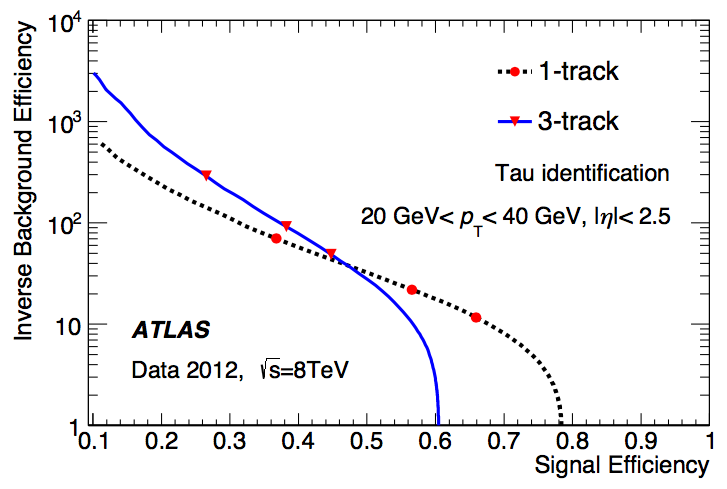
\includegraphics{figures/reconstruction/tau_5a}}
	}
	\hfill
	\subfloat[] {
		\resizebox{0.45\textwidth}{!}{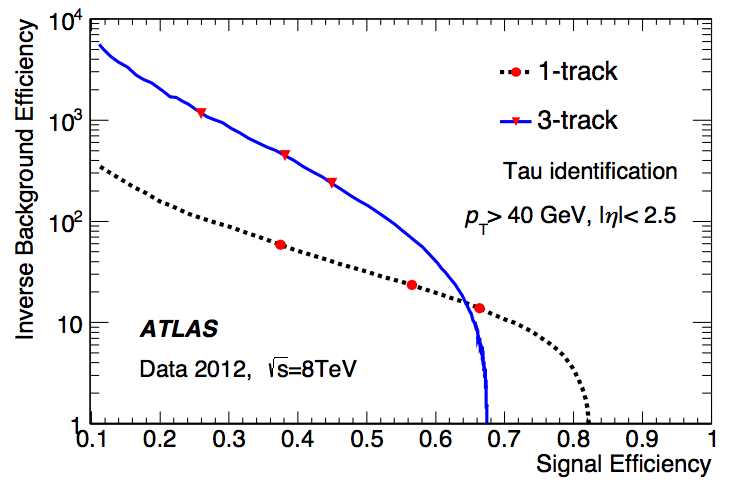
\includegraphics{figures/reconstruction/tau_5b}}
	}
	\caption{Inverse background efficiency (rejection power) versus signal efficiency for the BDT-based offline $\tau$ identification algorithm. (a) shows the efficiency for $\tau$ leptons with $\SI{20}{\giga\electronvolt}<\pt<\SI{40}{\giga\electronvolt}$, and (b) shows the efficiency for $\tau$ leptons with $\pt>\SI{40}{\giga\electronvolt}$. The three points on each curve correspond to the \texttt{BDT-tight}, \texttt{BDT-medium}, and \texttt{BDT-loose} working points, in order of increasing signal efficiency and decreasing background rejection power. The background consists of simulated multijet events, while the signal consists of simulated $Z$, $W$, and $Z'$ events decaying to $\tau$ leptons. }
	\label{fig:reco-tau-efficiency}
\end{figure}

\begin{figure}[htbp]
	\centering
	\resizebox{0.45\textwidth}{!}{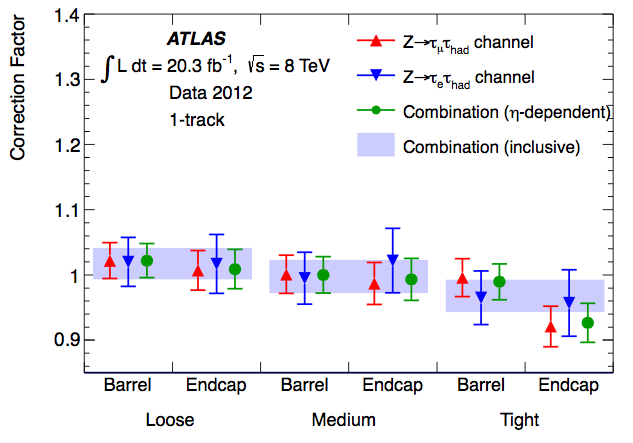
\includegraphics{figures/reconstruction/tau_11a}}
	\caption{Correction factors applied to simulation to equalize the efficiency to that measured in data, as measured in $Z$ tag-and-probe data. The error bars show the combined statistical and systematic uncertainty.}
	\label{fig:reco-tau-efficiency-scale-factors}
\end{figure}

\begin{figure}
	\centering
	\resizebox{0.6\textwidth}{!}{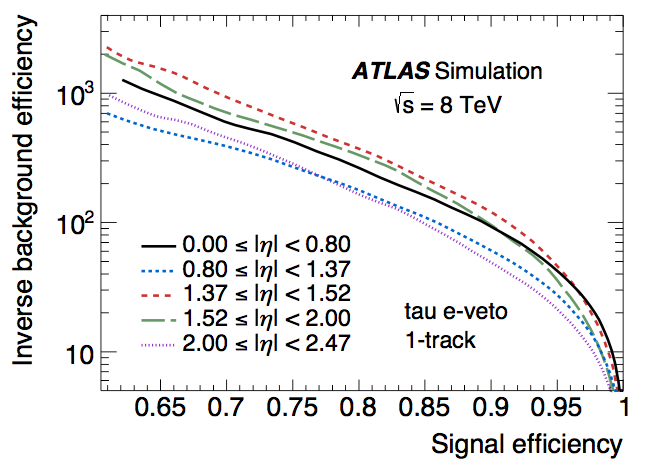
\includegraphics{figures/reconstruction/tau_9}}
	\caption{Electron rejection power versus 1-track $\tau_{\mathrm{had}}$ efficiency for the electron rejection BDT. }
	\label{fig:reco-tau-electron-rejection-efficiency}
\end{figure}

\subsection{Energy Scale and Resolution}\label{sec:reco-tau-energymomentum}
The hadronic $\tau$ reconstruction and identification are based on calorimeter cells calibrated at the local hadronic scale. Several corrections are applied to correct the energy to a $\tau$-specific energy scale (TES). First, corrections are derived using simulated $Z\rightarrow\tau\tau$, $W\rightarrow\tau\nu$, and $Z'\rightarrow\tau\tau$ events, generated with \pythia8. These corrections are determined as a function of the reconstructed $\tau_{\mathrm{had-vis}}$ energy and pseudorapidity based on the medium identification working point. A small pseudorapidity correction, reaching up to $|\Delta\eta|=0.01$, corrects a bias due to underestimated cluster energies in poorly-instrumented regions of the calorimeter. To account for pileup, $90$-$420 \MeV$ per additional reconstructed vertex is subtracted from the reconstructed $\tau_{\mathrm{had-vis}}$ energy, depending on $\eta$. The simulated $\tau_{\mathrm{had-vis}}$ energy resolution after these corrections is shown in figure~\ref{fig:reco-tau-energy-resolution}, and ranges between about $20\%$ at very low energy to about $5\%$ above a few hundred GeV.

\begin{figure}[htbp]
	\centering
	\resizebox{0.6\textwidth}{!}{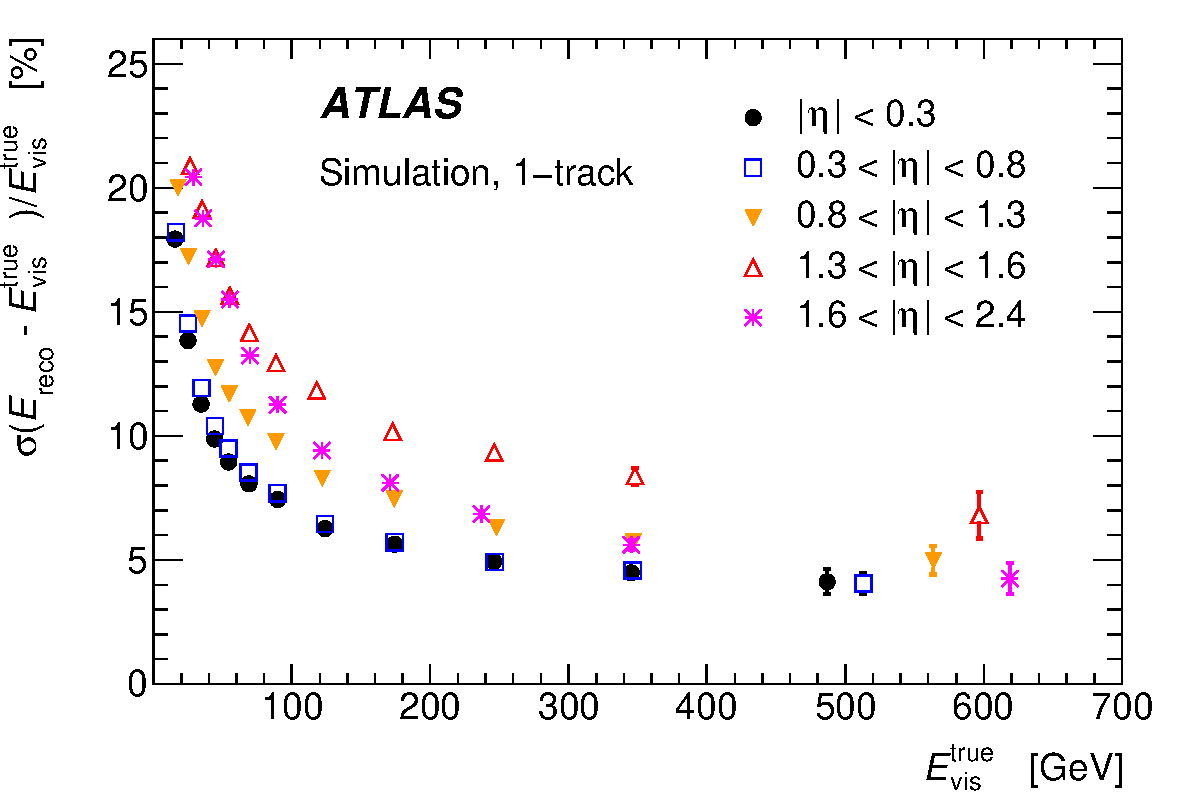
\includegraphics{figures/reconstruction/tau_fig_16a}}
	\caption{Energy resolution for hadronically decaying $\tau$ leptons with one associated track in various pseudorapidity regions. The resolution is the standard deviation of a Gaussian fit to the distribution of $\frac{E_{\mathrm{reco}}-E_{\mathrm{true-vis}}}{E_{\mathrm{true-vis}}}$ in bins of $E_{\mathrm{true-vis}}$ and $|\eta_{\mathrm{true-vis}}|$.}
	\label{fig:reco-tau-energy-resolution}
\end{figure}


Finally, data-driven corrections and systematic uncertainties on the $\tau$ energy scale are derived using a \emph{deconvolution} method~\cite{TheATLASCollaboration:2011ks}. The method combines the systematic uncertainties on the single-particle response of the calorimeters based on the well-known branching fractions of hadronically decaying $\tau$ leptons. A TES correction of about $1\%$ is determined. Including additional systematic uncertainties covering the detector modeling, pileup, non-closure of the calibration method, and the hadronic shower model, the total TES uncertainty is $2-3\%$ for one-prong decays and $2-4\%$ for three-prong decays.

\section{Jets}\label{sec:reco-jets}
Jets play an important complementary role to leptons in the analyses described in the following chapters. The new physics scenarios considered often produce jets in addition to the three required leptons. If the new particles are colored, as in strongly produced supersymmetry, then high-$\pt$ jets can be produced in cascade decays. Alternatively, if the new particles decay via the weak interaction, then the decays will often contain hadronically decaying weak bosons. From the background point of view, due to the colored initial state in $pp$ collisions, jets are produced copiously at the LHC. Despite the stringent lepton identification cuts, jets misidentified as leptons or containing semileptonic decays can constitute a significant source of backgrounds to trilepton final states.

The reconstruction of jets in the calorimeter is based on topological clusters of energy~\cite{TheATLASCollaboration:2011ks,TheATLASCollaboration:2015ds}. The reconstruction steps are shown in figure~\ref{fig:reco-jet-reconstruction-flowchart}. Clusters are formed by grouping together calorimeter cells based on their signal-to-noise ratio, $S/N$, where the $N$ includes electronic noise and contributions from pileup interactions. Cells with $S/N>4$ form the cluster seeds, which are then expanded to include all connected cells with $S/N>2$. Finally, cells along the perimeter with $S/N>0$ are added to the cluster. The cluster energies are then calibrated according to one of two scales: the electromagnetic (EM) scale assumes that the cell energy is due to an electromagnetic shower, while the local cell signal weighting (LCW) method classifies energy deposits as electromagnetic or hadronic in origin. The jets used in this dissertation are constructed from cells calibrated at the LCW scale.

\begin{figure}[htbp]
	\centering
	\resizebox{0.8\textwidth}{!}{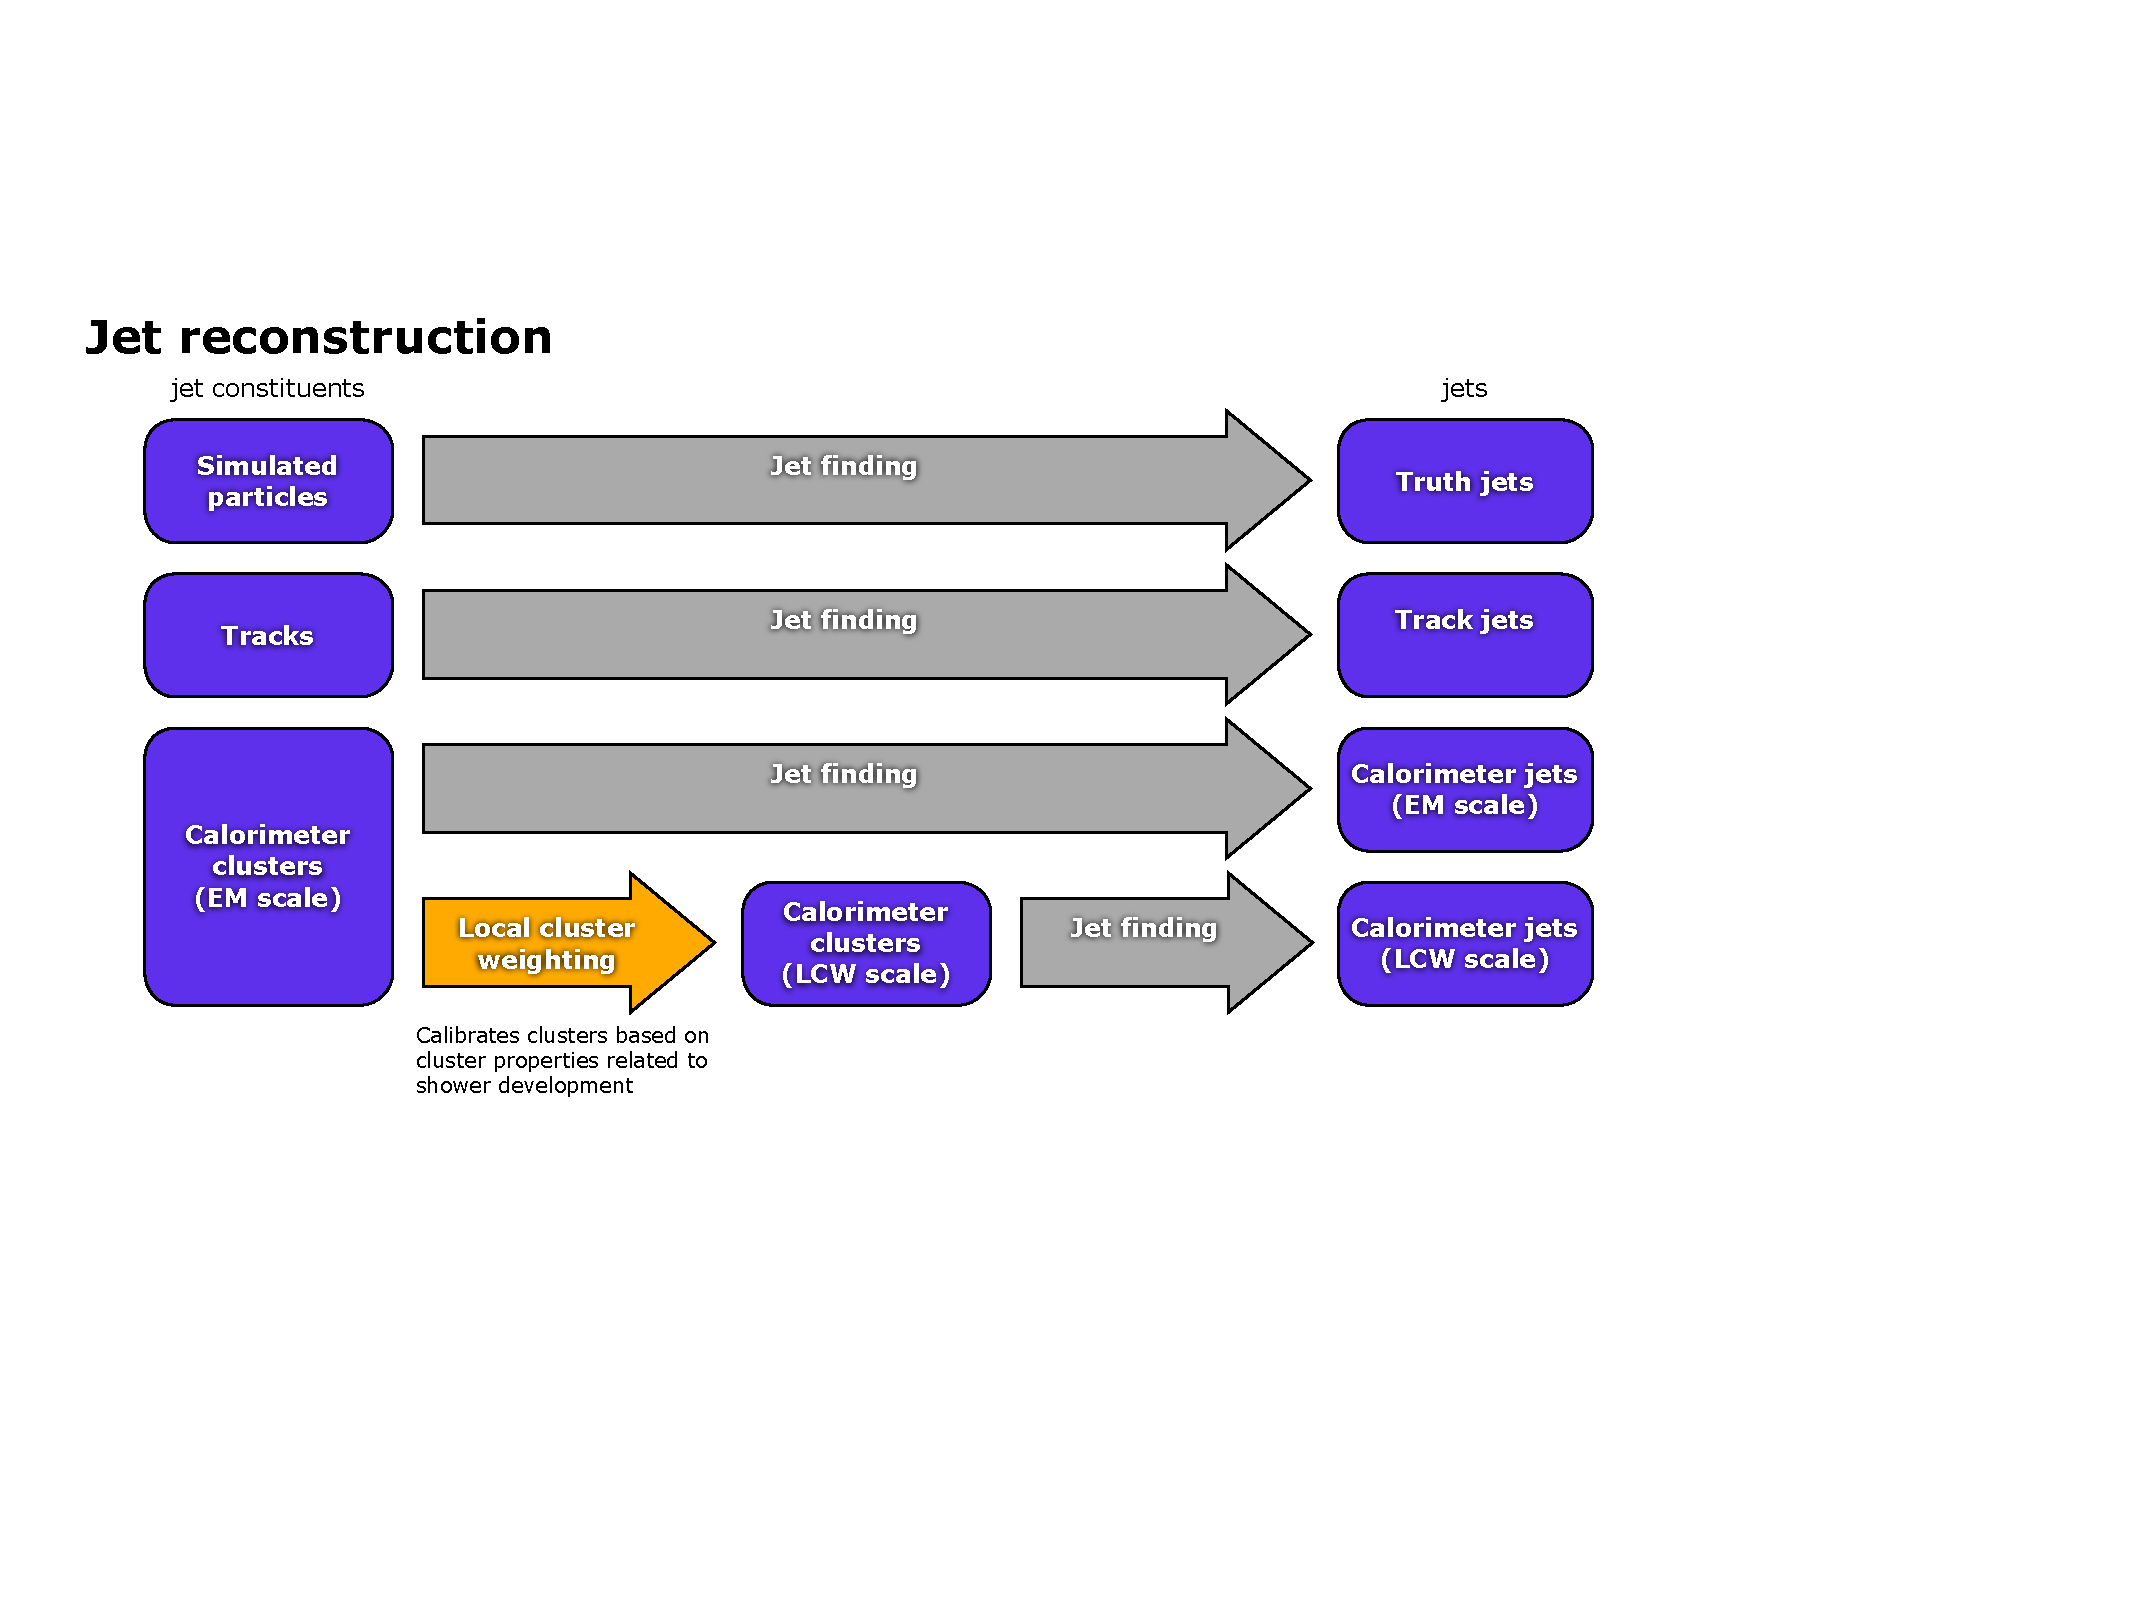
\includegraphics{figures/reconstruction/jet_02}}
	\caption{Overview of the jet reconstruction, showing the inputs to and outputs from the jet finding algorithms. The bottom two rows show the reconstruction of calorimeter jets, while the top two rows show jets built from truth particles in simulation and from tracks.}
	\label{fig:reco-jet-reconstruction-flowchart}
\end{figure}


Next, the jet finding algorithms group the calibrated clusters into collections of jets. The algorithm used in this dissertation is the anti-$k_{\mathrm{t}}$ algorithm with a distance parameter of $R=0.4$, implemented in \textsc{FastJet}~\cite{Cacciari:2008gp,Cacciari:2011ma}. A distance measure between objects, $d_{i,j}$, and between objects and the beam, $d_{i,B}$, is defined as
%Cacciari:2012br - what was this?

\begin{align}
	d_{i,j} &= \mathrm{min}(k_{\mathrm{t}, i}^{2p}, k_{\mathrm{t}, j}^{2p}) \frac{\Delta_{ij}^2}{R^2}, \\
	d_{i,B} &= k_{\mathrm{t},i}^{2p},
\end{align}

where $k_{\mathrm{t,i}}$ is the transverse momentum of object $i$, $\Delta_{i,j}=\sqrt{(y_i-y_j)^2+(\phi_i-\phi_j)^2}$ is the geometrical distance in rapidity ($y_{i,j}$) and azimuthal angle ($\phi_{i,j}$), and $p$ is a parameter that controls the relative importance of energy versus geometrical ($\Delta_{ij}$) scales, taken to be $p=-1$ for the anti-$k_{\mathrm{t}}$ algorithm. The algorithm combines objects sequentially by considering the smallest distance in the event. If the smallest distance is between two objects $i$ and $j$, then the objects are combined. If the smallest distance is between object $i$ and the beam $B$, then $i$ is classified as a jet and removed from the object list. The algorithm continues until there are no objects left. 

Loose quality cuts are applied to reject events with jets due to non-collision sources, such beam-gas collisions between protons in one beam and the residual gas in the beam pipe, beam-halo events due to collisions with upstream collimators, muons from cosmic rays, and calorimeter noise. The cuts have an efficiency of above 99.8\% for retaining real jets. 


\subsection{Energy Scale and Resolution}\label{sec:reco-jets-energy-scale-resolution}
The jet energy is calibrated in several steps, as shown in figure~\ref{fig:reco-jet-calibration-flowchart}. First, pileup and origin corrections are applied. Energy contributions from pileup interactions in the same or nearby bunch crossings are subtracted based on simulation, with the correction determined in bins of jet $\pt$ and $\eta$ as a function of the number of reconstructed vertices in the event and the average number of interactions per crossing expected from the instantaneous luminosity. 
%the jet area, and the median $\pt$ density of jets in the event. 
The geometry of the jet is corrected to point from the primary event vertex, rather than the nominal center of the ATLAS detector. 

\begin{figure}[htbp]
	\centering
	\resizebox{0.8\textwidth}{!}{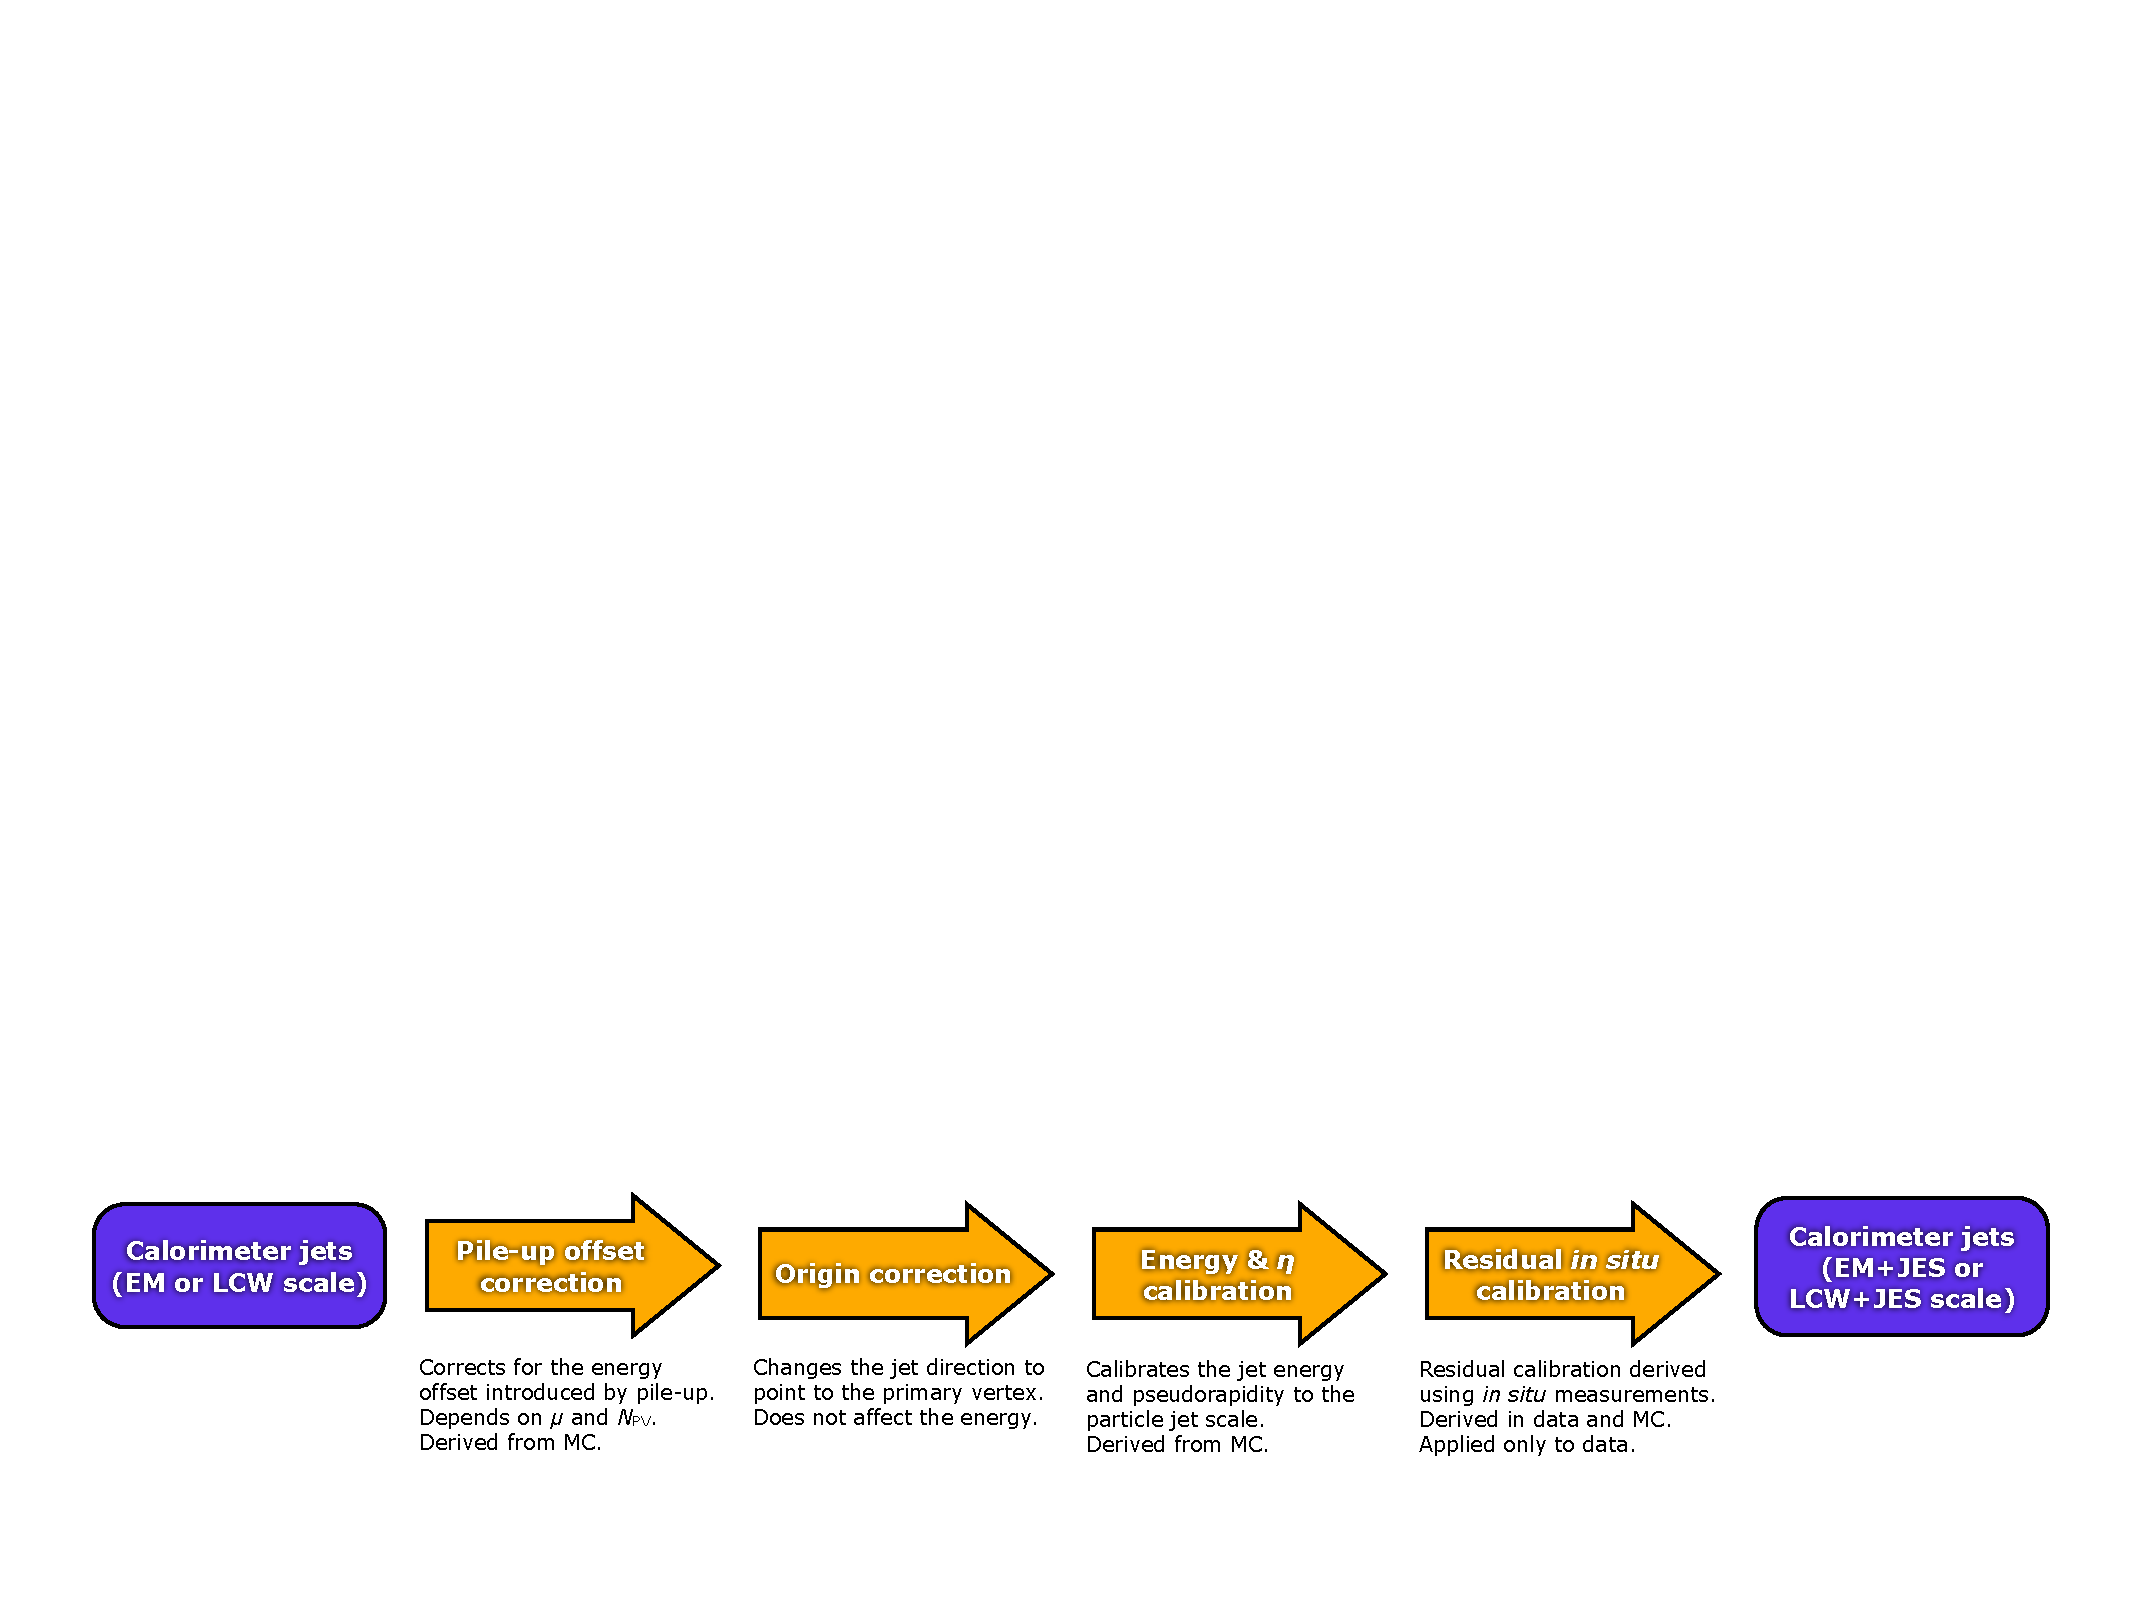
\includegraphics{figures/reconstruction/jet_03}}
	\caption{Overview of the jet calibration scheme. }
	\label{fig:reco-jet-calibration-flowchart}
\end{figure}


The energy and pseudorapidity of the jet are initially calibrated based on the relationship between jets reconstructed from calorimeter clusters and jets reconstructed from truth particles in simulation. Then, in situ corrections are applied to the calibrated jets to correct for effects not described by the initial simulation-based calibration. The corrections are based on balancing the transverse momenta of jets against other well-calibrated objects. Jets in the central region, with detector rapidity $|\eta_{\mathrm{det}}|<1.2$, are calibrated against photons and leptonically decaying $Z$ bosons. Jets with high transverse momentum, $\pt>210 \GeV$, are also calibrated using multijet events, balancing the high-$\pt$ jet against several low-$\pt$ jets. Jets with $1.2<|\eta_{\mathrm{det}}|<2.8$ are calibrated against central jets with $|\eta_{\mathrm{det}}|<0.8$; due to a lack of statistics with which to derive the calibration, more forward jets, with $\pm2.8<\eta_{\mathrm{det}}<4.5$, are assigned the same calibration as jets with $\eta_{\mathrm{det}}=\pm2.8$. The in situ calibrations shift the jet energy in data down by about $2\%$ for $\pt<100 \GeV$, and decreases with increasing $\pt$. 

A large number of systematic uncertainties are assigned to the in situ calibration procedure, related to the modeling of the detector and physics processes in simulation and to the in situ methods themselves. The uncertainties are summarized in figure~\ref{fig:reco-jes-uncertainty}. Additionally, systematic uncertainties related to the pileup correction, high-$\pt$ jets, jet flavor, and differences simulation settings are assigned where appropriate.

\begin{figure}[htbp]
	\centering
	\subfloat[ $\eta=0.5$] {
		\resizebox{0.45\textwidth}{!}{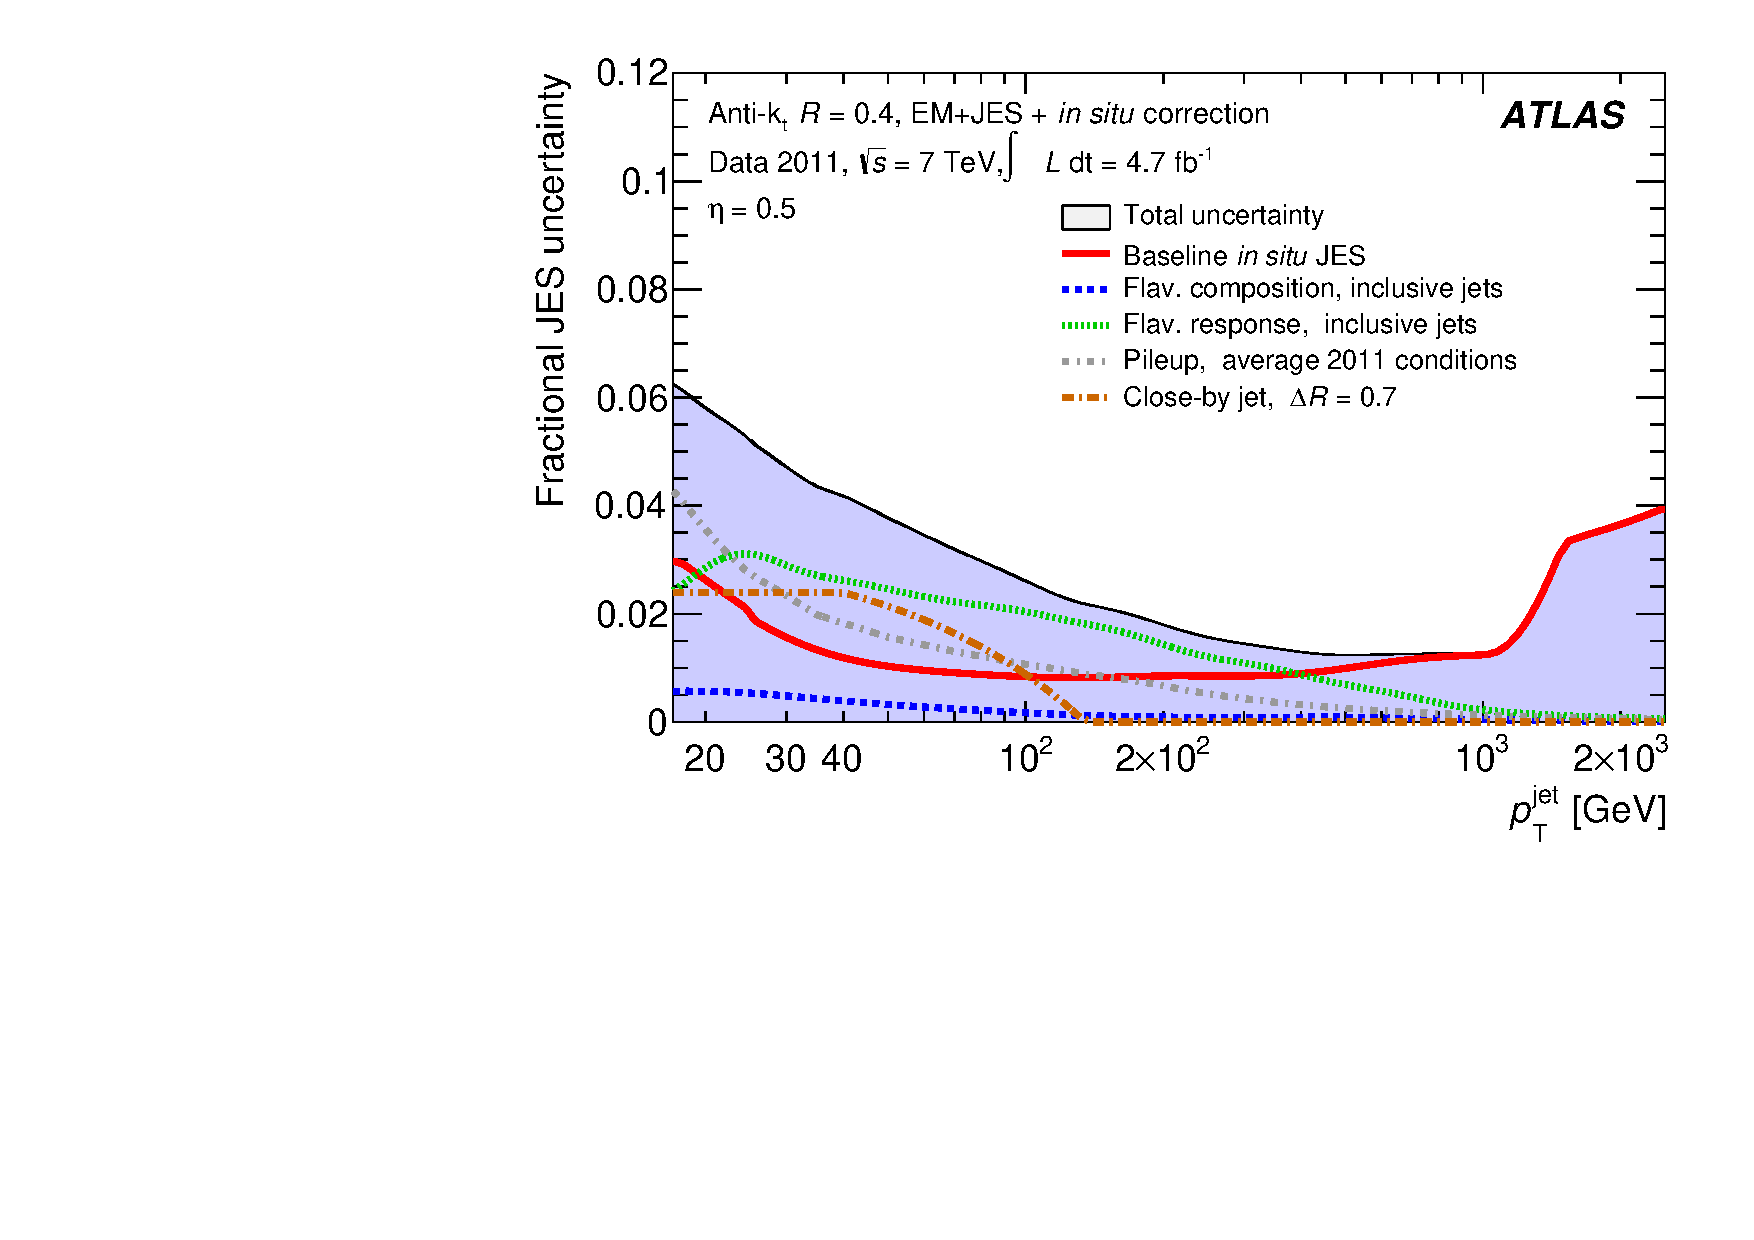
\includegraphics{figures/reconstruction/jet_64a}}
	}
	\hfill
	\subfloat[ $\eta=2.0$] {
		\resizebox{0.45\textwidth}{!}{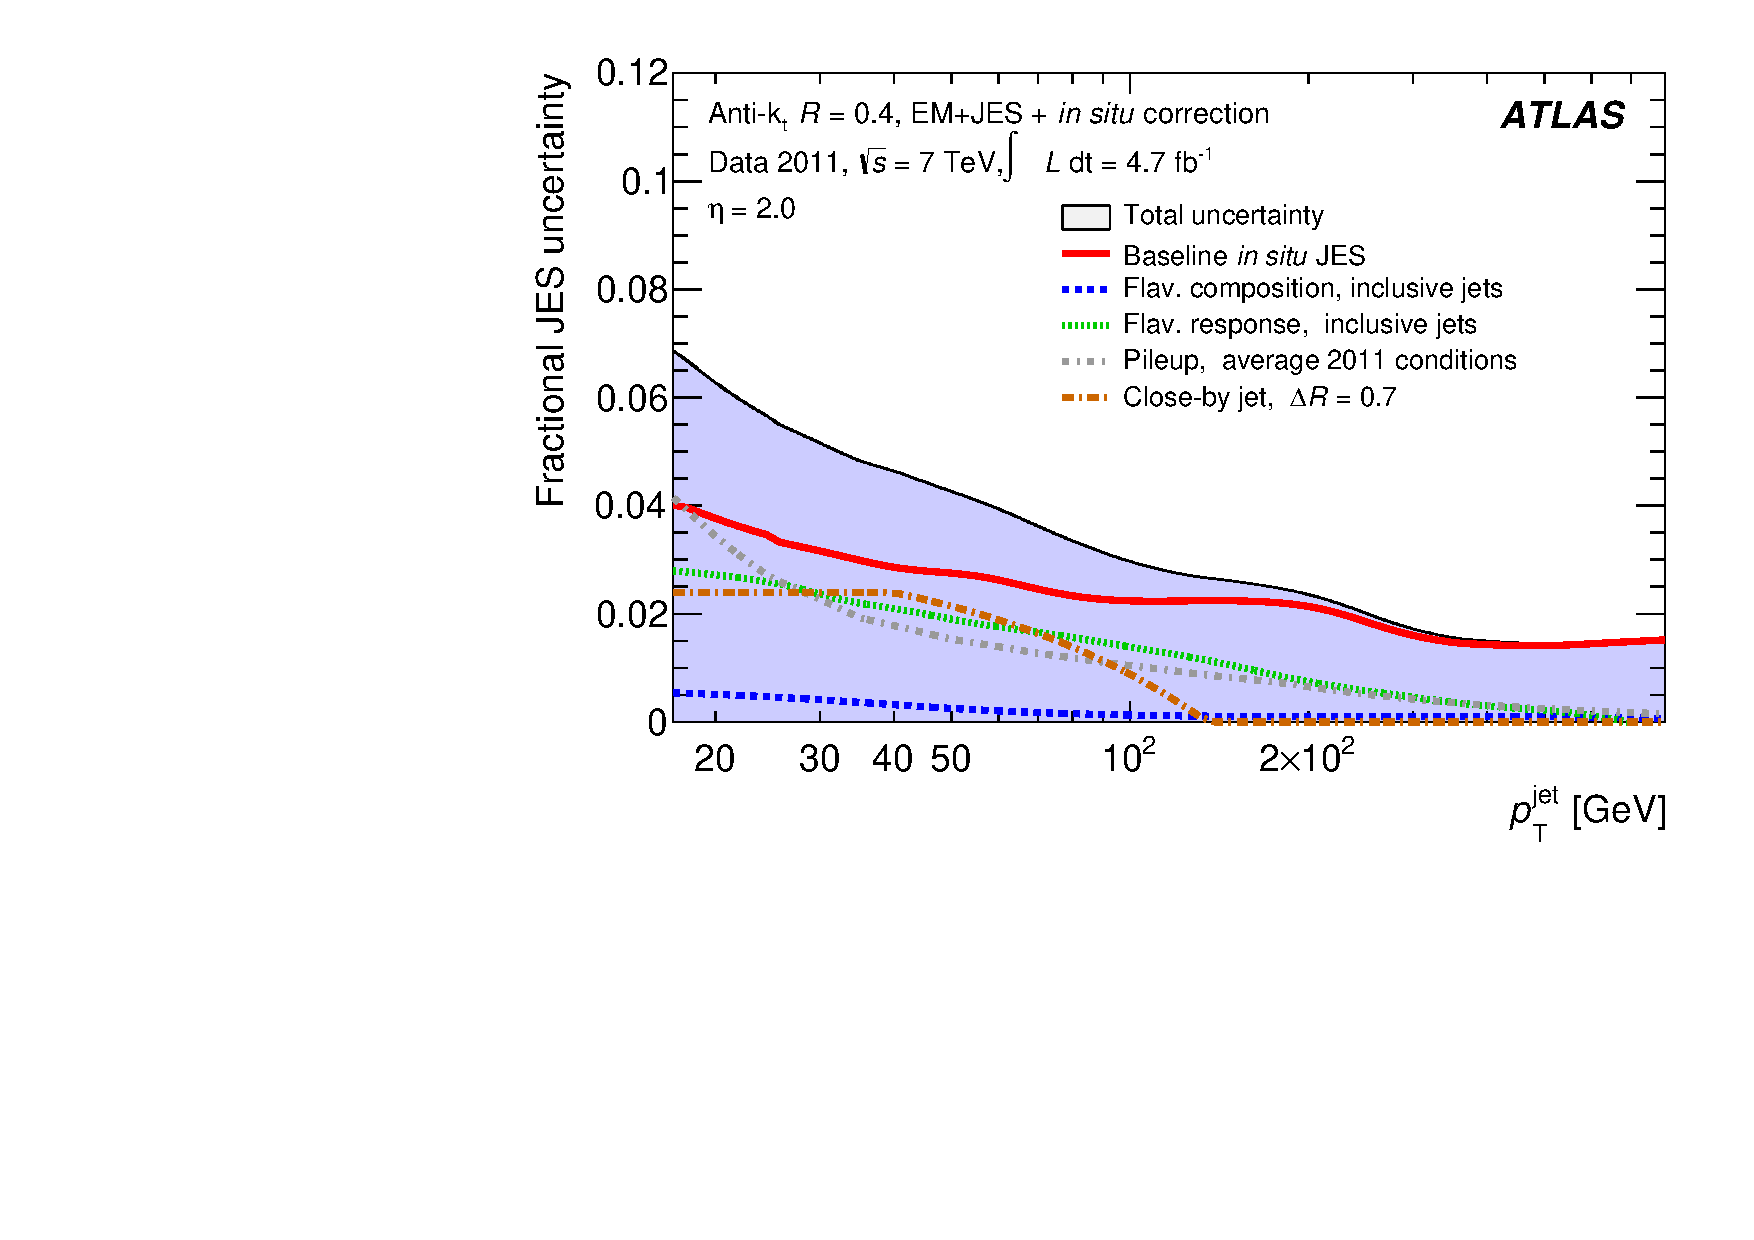
\includegraphics{figures/reconstruction/jet_64b}}
	} \\
	\subfloat[ $\pt^{\mathrm{jet}}=\SI{25}{\giga\electronvolt}$] {
		\resizebox{0.45\textwidth}{!}{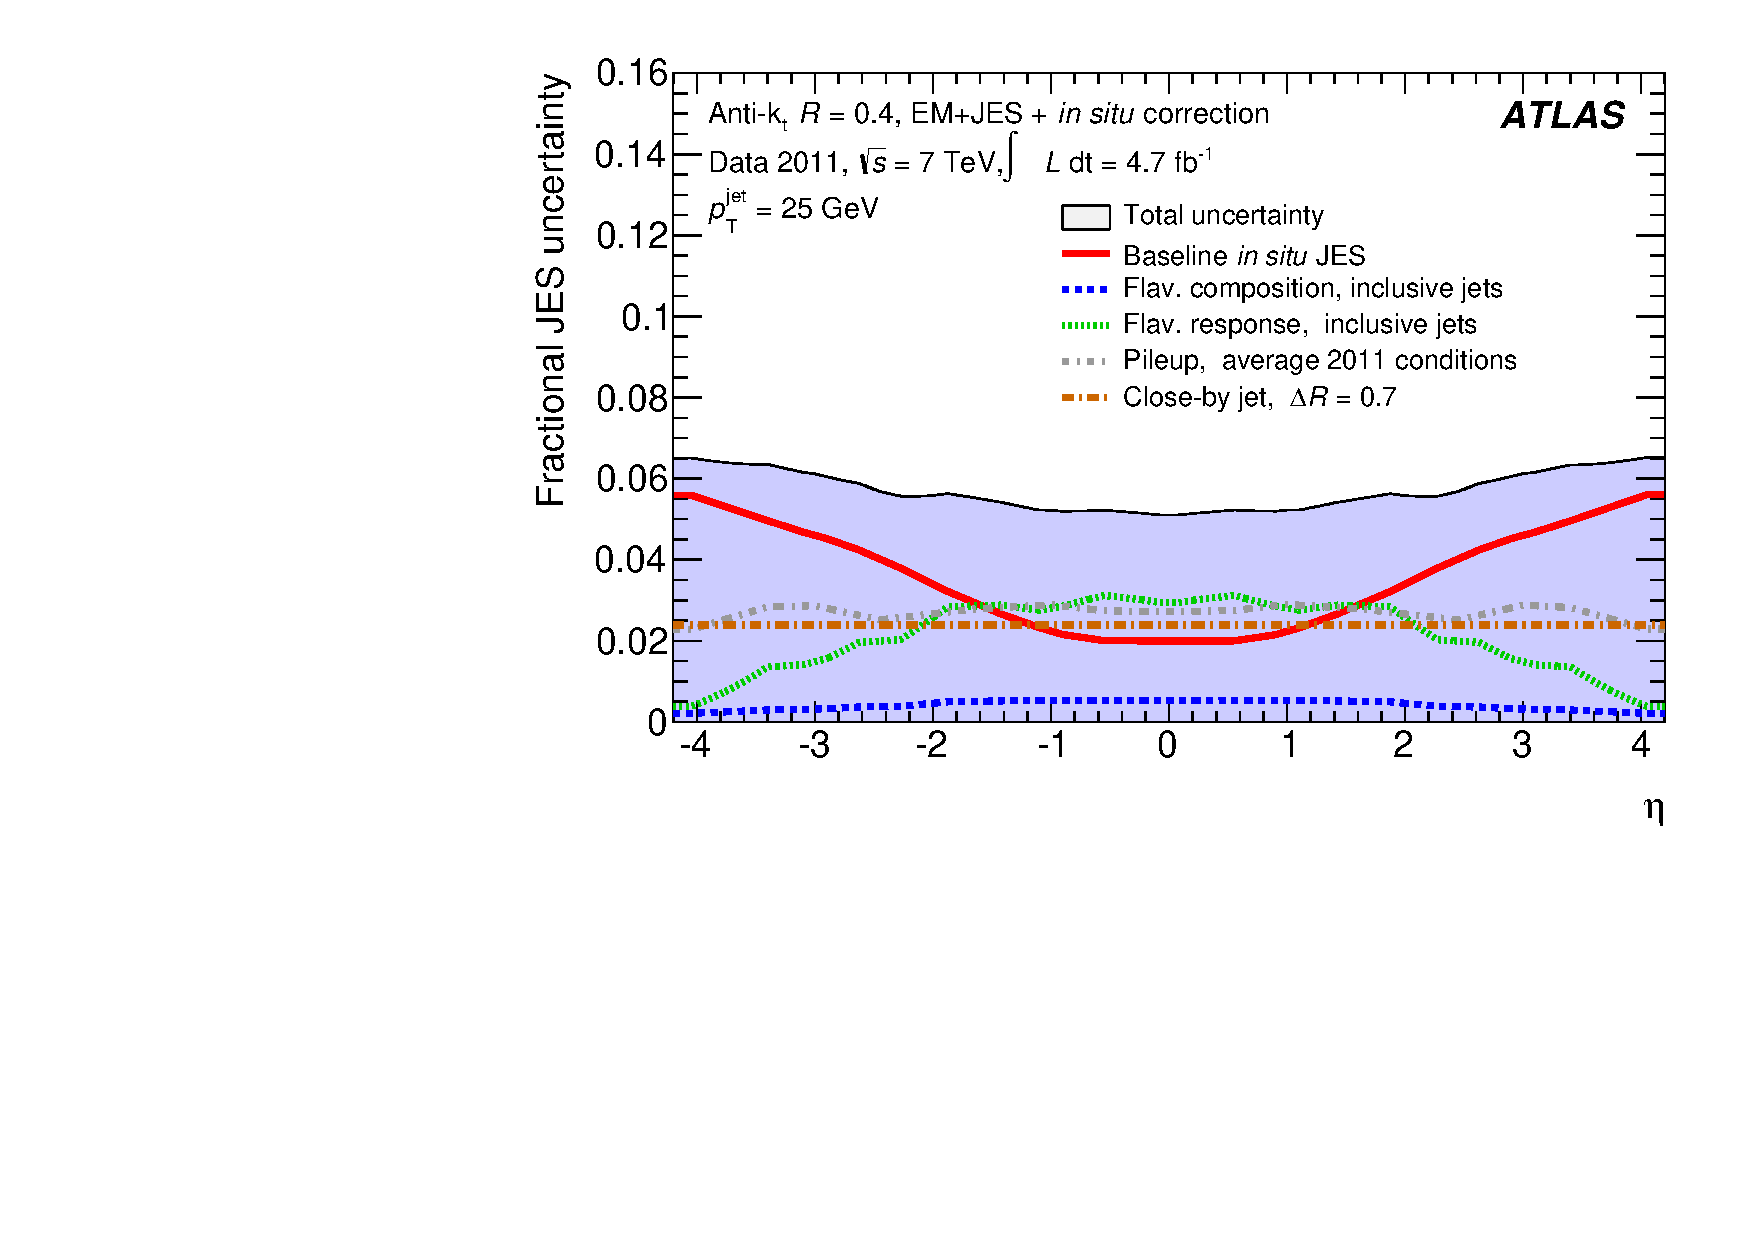
\includegraphics{figures/reconstruction/jet_64c}}
	}
	\hfill
	\subfloat[ $\pt^{\mathrm{jet}}=\SI{300}{\giga\electronvolt}$] {
		\resizebox{0.45\textwidth}{!}{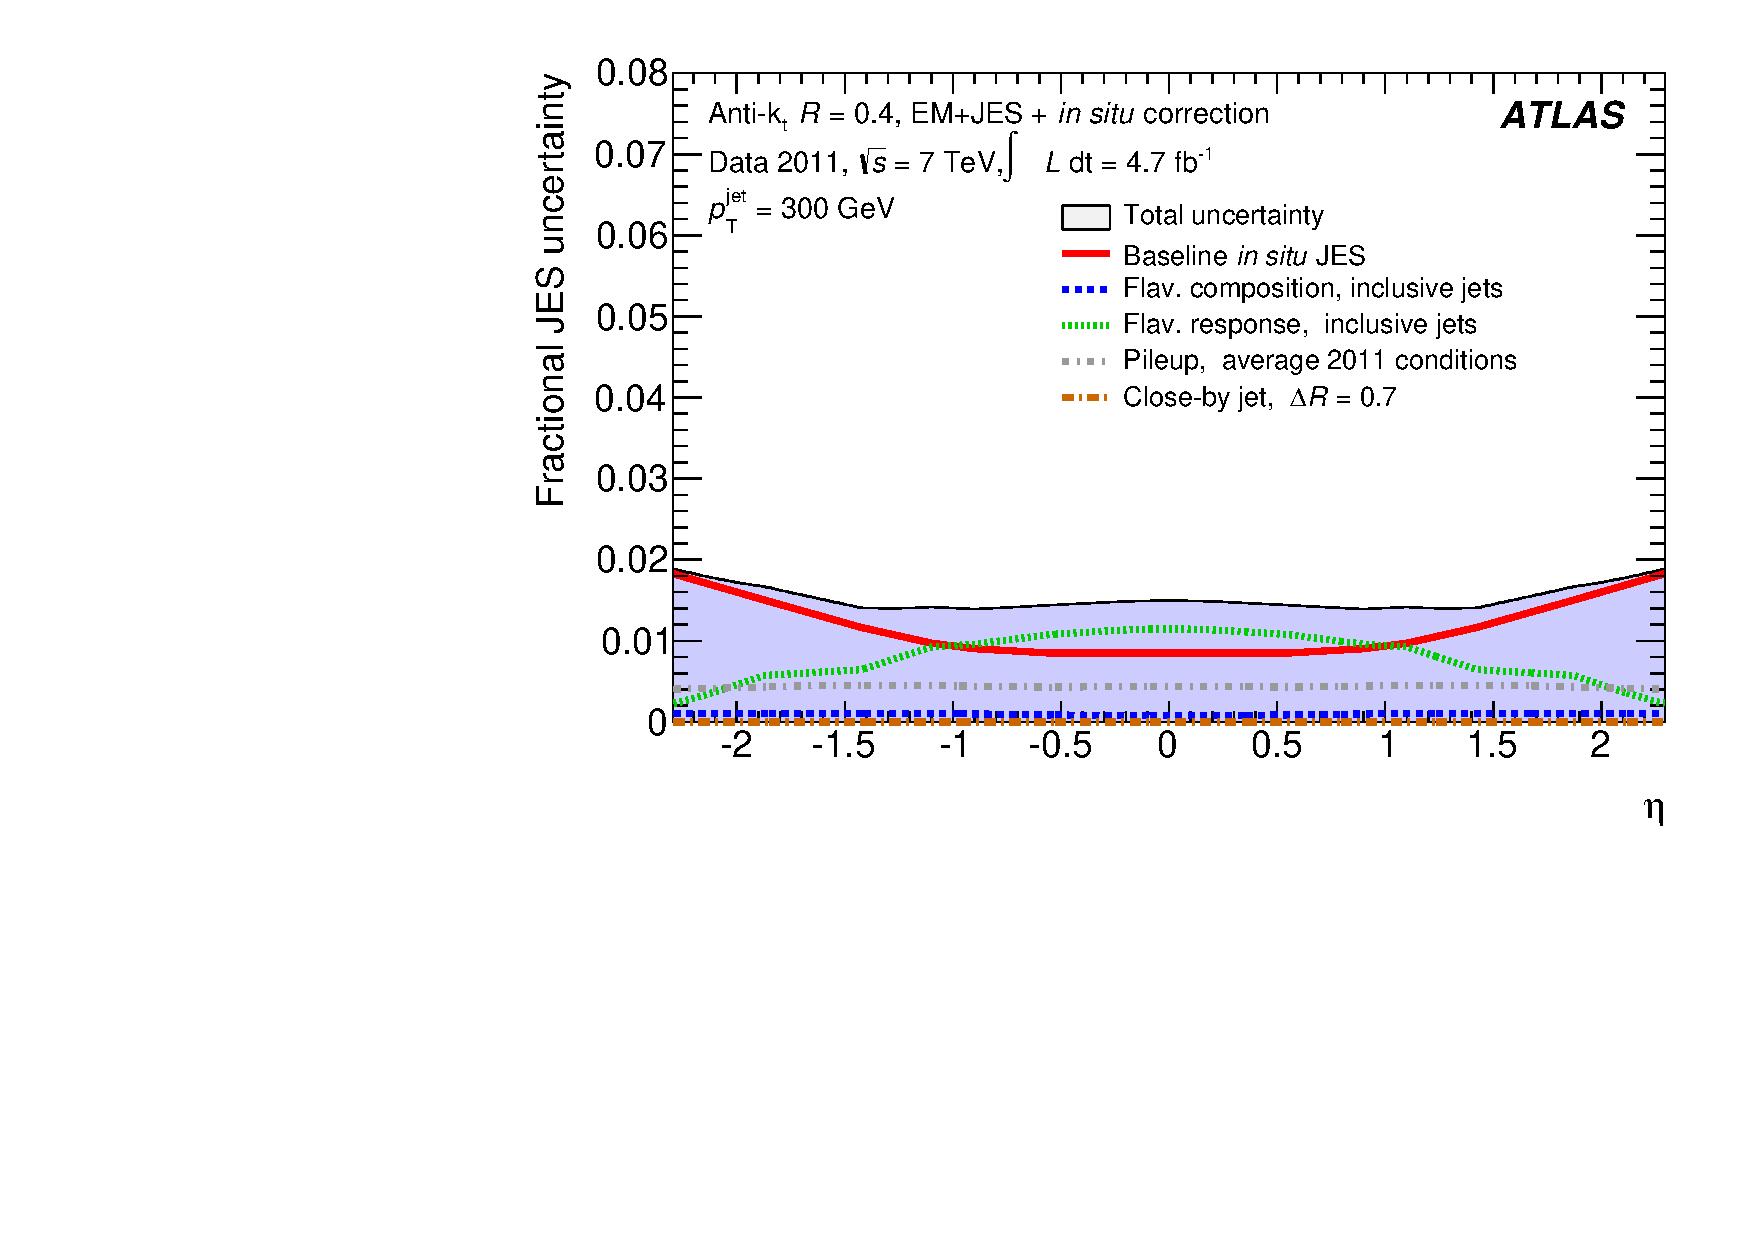
\includegraphics{figures/reconstruction/jet_64d}}
	} \\
	\caption{Sample-dependent fractional jet energy scale (JES) systematic uncertainty as a function of $\pt^{\mathrm{jet}}$ (top) and $\eta$ (bottom), at fixed values of $\eta$ or $\pt^{\mathrm{jet}}$, respectively. The jets are reconstruction using the anti-$k_{\mathrm{T}}$ algorithm with a radius parameter of $R=0.4$ from clusters at the LCW scale, and are calibrated as described in the text. The shaded area shows the total systematic uncertainty, while the colored lines show the contribution of various individual sources of uncertainty.}
	\label{fig:reco-jes-uncertainty}
\end{figure}

\subsection{Pileup Suppression}\label{sec:reco-jets-jvf}
Jets due to pileup interactions can be suppressed using the track information, at the cost of introducing some pileup-dependence to the jet reconstruction inefficiency. For a given jet and primary vertex, the \emph{jet vertex fraction} (JVF) is defined as the ratio of the $\sum \pt$ of tracks associated with the jet and matched to the primary vertex to the $\sum\pt$ of all tracks associated to the jet, shown schematically in figure~\ref{fig:jvf-cartoon}. Specifically, letting $\mathcal{T}$ be the set of tracks associated to the jet, the JVF is defined as:

\begin{equation}\label{eqn:jvf}
	\mathrm{JVF}=\frac{\sum_{i\in\mathcal{T}} p_{\mathrm{T},i} \Theta_V(i)} {\sum_{i\in\mathrm{jet}} p_{\mathrm{T},i} },
\end{equation}

where $\Theta_V(i)=1$ if the track $i$ is matched to the primary vertex and $0$ otherwise. If $\mathcal{T}$ is empty, then $\mathrm{JVF}\equiv -1$. In this dissertation, the primary vertex is chosen as the vertex with the highest $\sum \pt^2$ of tracks, and $\mathrm{JVF}>0.5$ is required for jets with $20 \GeV<\pt<50 \GeV$. 

\begin{figure}[htbp]
	\centering
	\resizebox{0.6\textwidth}{!}{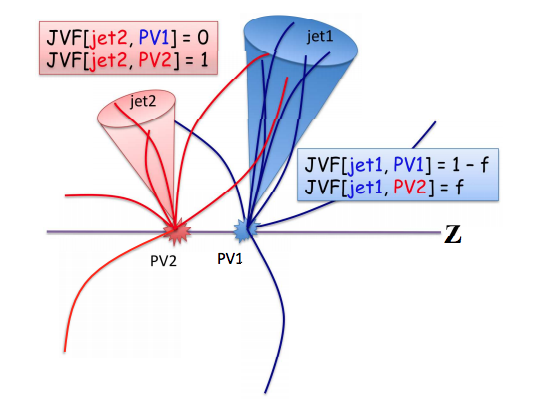
\includegraphics{figures/reconstruction/jvf_cartoon.png}}
	\caption{Schematic representation of the jet vertex fractions in the case of two jets and two primary vertices. $f$ is the fraction of track $\pt$ in jet 1 due to tracks associated with vertex PV2.}
	\label{fig:jvf-cartoon}
\end{figure}


\subsection{$b$-tagging}\label{sec:reco-bjets}
The model-independent trilepton analysis (chapter~\ref{ch:model-independent-trilepton-search}) also makes use of the tagging of jets due to $b$ quarks. Jets containing $b$ quarks have several features which distinguish them from jets due to light quarks or gluons. $B$ hadrons have proper decay lengths of approximate $0.5 \mm$, long enough to be observed in the form of tracks or vertices reconstructed away from the primary interaction point. They also have large masses compared to other hadrons, leading to wider jets with more particles. 

The algorithm used to tag $b$-jets is an artificial neural network called the MV1 algorithm~\cite{TheATLASCollaboration:2014vj}. The neural network uses three simpler likelihood-based algorithms as inputs~\cite{TheATLASCollaboration:2009ut,TheATLASCollaboration:2011wh}: 

\begin{itemize}
	\item \textbf{IP3D}: Uses the transverse and longitudinal impact parameters of the tracks associated with a jet.
	\item \textbf{SV1}: Attempts to reconstruct a secondary vertex from the tracks associated with a jet. The most sensitive variable is the decay length significance between the secondary vertex and the primary event vertex. Additionally, the algorithm uses the invariant mass of tracks associated with the secondary vertex, the ratio of the energy of tracks assigned to the vertex to the energy of all tracks within the jet, and the number of two-track vertex candidates within the jet. 
	\item \textbf{JetFitter}: Constructs a line connecting the primary vertex with one or more points associated with $b$- or $c$-hadron decays using a Kalman filter. The algorithm makes use of variables similar to the SV1 algorithm, along with the flight length significance between decays. Note that the algorithm does not require secondary vertices, allowing for the identification of decays with only one track. 
\end{itemize}

The MV1 algorithm is trained on simulated data, using $b$-jets as signal and light quark jets as background, and returns a tag weight for each jet. The tag weight is used to establish working points with a given signal efficiency and background rejection power, as shown in figure~\ref{fig:reco-b-tagging-efficiency-rejection}. The model-independent trilepton analysis uses the working point with $80\%$ signal efficiency. The performance of the algorithm as a function of transverse momentum is shown in figure~\ref{fig:reco-b-tagging-efficiency-pt}.

\begin{figure}[htbp]
	\centering
	\subfloat[] {\label{fig:reco-b-tagging-efficiency-rejection}
		\resizebox{0.45\textwidth}{!}{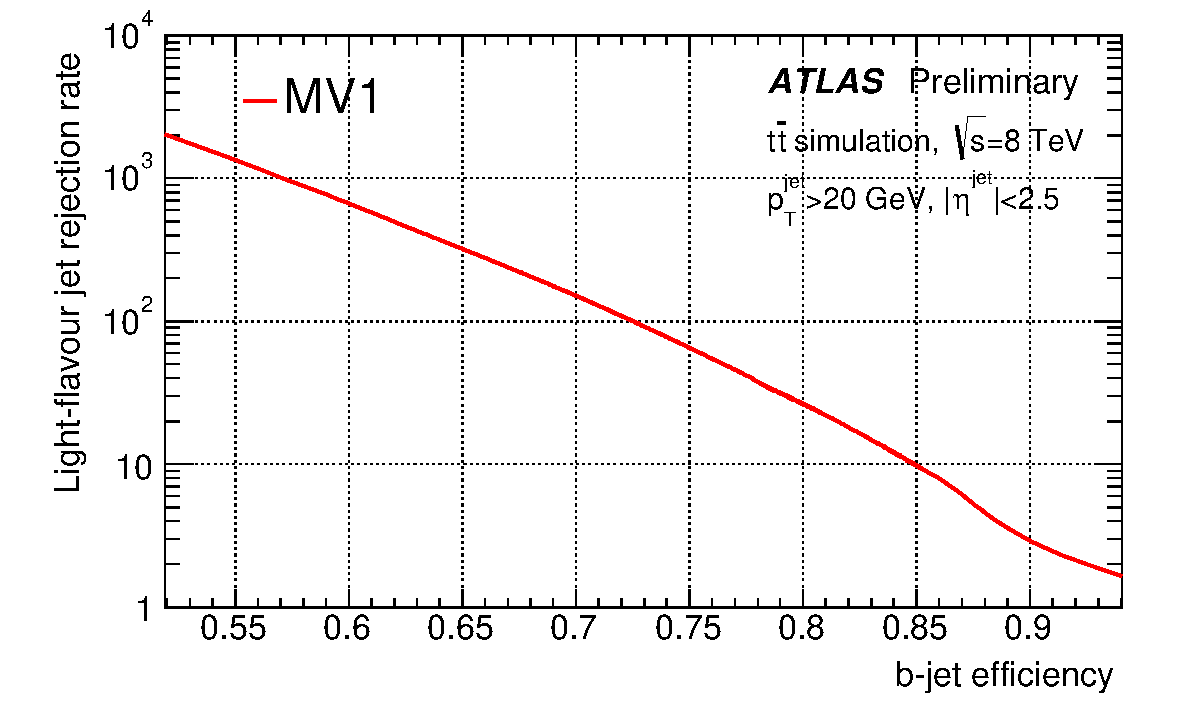
\includegraphics{figures/reconstruction/btag_fig_01}}
	}
	\hfill
	\subfloat[] {\label{fig:reco-b-tagging-efficiency-pt}
		\resizebox{0.45\textwidth}{!}{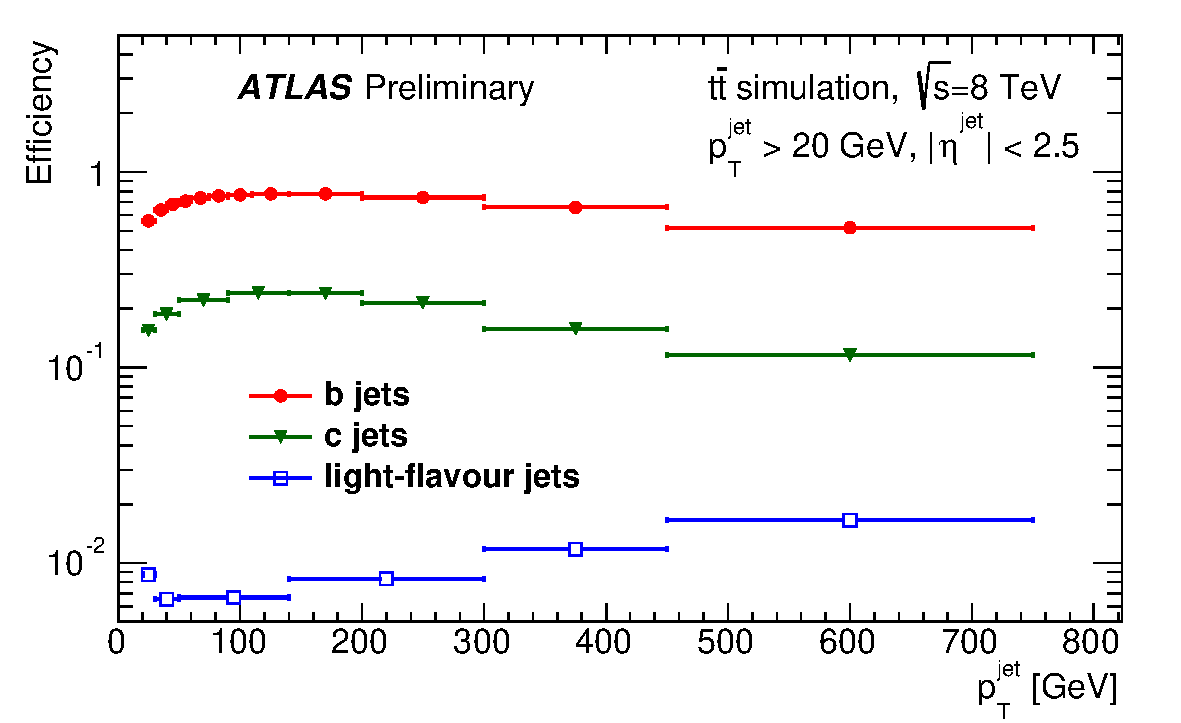
\includegraphics{figures/reconstruction/btag_fig_02a}}
	}
	\caption{Performance of the MV1 $b$-tagging algorithm. The inclusive signal efficiency versus background rejection is shown at left. The signal and background efficiencies at the 70\% working point are shown as a function of $\pt$ at right.}
	\label{fig:reco-b-tagging-efficiency}
\end{figure}


\section{Invisible Particles}\label{sec:reco-met}
Neutrinos interact only via the weak interaction, and hence escape the detector without interacting with any of the detector components. The same is true for any new stable, neutral, and colorless particles, such as the lightest supersymmetric particle in $R$ parity-conserving scenarios or sterile neutrinos. The presence of such particles can only be inferred through the overall imbalance of the transverse momentum\footnote{The longitudinal momentum imbalance, $E_{z}^{\mathrm{miss}}$, is not useful in $pp$ collisions due to the unknown longitudinal momenta of the initial colliding partons.} of the other visible collision products, $\metvec=(E_{x}^{\mathrm{miss}},\,E_{y}^{\mathrm{miss}}$. 

The missing transverse momentum is defined as the negative vector sum of the visible objects in the event~\cite{TheATLASCollaboration:2012jy,TheATLASCollaboration:2013ua}. The energies are mostly determined from calorimeter measurements, except for muons. To avoid using calorimeter energy deposits multiple times, the algorithm assigns energy to deposits to a single object according to a strict order: electrons are identified first, followed by photons, hadronically decaying $\tau$ leptons, jets, and muons. Depending on the analysis requirements, the energy of a given physics object can be determined using the full reconstruction algorithm, or the energy deposits can be calibrated to the EM or LCW scales. Finally, topological clusters and tracks not assigned to physics objects are included in $\metvec$ calculation as the so-called soft term. The missing transverse energy is given by:

\begin{equation}\label{eqn:reco-met}
	E_{x(y)}^{\mathrm{miss}} = -\left(E_{x(y)}^{e} + E_{x(y)}^{\gamma} + E_{x(y)}^{\tau} + E_{x(y)}^{\mathrm{jets}} + E_{x(y)}^{\mu} + E_{x(y)}^{\mathrm{soft}}\right),
\end{equation}

where each term on the right represents the total momentum of the reconstructed objects in the $x$ or $y$ directions.

The measured $\metvec$ receives contributions from sources besides invisible particles, including calorimeter noise, particles falling in insensitive regions of the detector, energy mismeasurements, and pileup interactions. These effects are mitigable to varying degrees. Particles falling outside the detector acceptance contribute irreducibly to the $\metvec$ resolution. For physics objects like electrons or jets, the noise and pileup contributions are suppressed by the reconstruction algorithms and identification cuts. To reduce the noise and pileup contributions to the soft term, the cells are grouped into topological clusters. Rejecting events where the $\metvec$ is parallel or antiparallel to the physics objects can mitigate the impact of energy mismeasurements. 


\section{Object Selection}\label{sec:model-independent-object-definitions}
The analyses described in this dissertation search for energetic leptons and jets produced in the decays of new heavy particles. The leptons and jets typically have large transverse momenta and are well-separated from other objects in the event, due to the large difference in the mass scale between the final decay products (leptons or hadrons with mass $m\lesssim\SI{10}{\giga\electronvolt}$) and the parents ($W/Z$ bosons or the new particles themselves, with mass $m\gtrsim\SI{80}{\giga\electronvolt}$). The new particles typically have short lifetimes, and hence the leptons and jets are produced promptly at the location of the initial proton-proton interaction, consistent with originating from the selected primary vertex. These properties can be used to suppress backgrounds due to Standard Model processes and detector effects, described in chapter~\ref{ch:backgrounds}. 

\subsection{Leptons}\label{sec:model-independent-lepton-definitions}

The events used in this dissertation are required to have at least three reconstructed electrons, muons, or hadronically decaying $\tau$ leptons. A summary of the lepton selections is shown in tables~\ref{table:electron-muon-selections} and \ref{table:tau-selections}. Leptons are required to satisfy the following requirements:

\begin{itemize}

	\item \textbf{Transverse momentum}: Electrons and muons must have $\pt>15 \GeV$, while hadronically decaying $\tau$ leptons must have $\pt>20 \GeV$. The transverse momentum cut is driven by the availability of triggers with which to perform data-driven estimates of backgrounds due to sources like semileptonically decays in jets or misidentified jets (see section~\ref{sec:fake-factor-method}). 

	\item \textbf{Geometrical acceptance}: Electrons are required to have $|\eta|<2.47$, excluding the transition region $1.37<|\eta|<1.52$ between the barrel and end-cap calorimeters. Muons and $\tau$ leptons are required to have $|\eta|<2.5$.

	\item \textbf{Particle identification}: To suppress the reducible backgrounds, the leptons must satisfy strict requirements related to particle identification. Electrons candidates must satisfy the \texttt{tight++} set of identification cuts. Electrons are neglected if they fall in a region affected by the presence of a dead front end board in the first or second sampling layer, a dead high voltage supply, or a masked cell in the core. Muons are required to be \emph{combined}, with associated hits in the inner detector and muon spectrometer. Specifically, associated inner detector track must have:
	\begin{itemize}
	  \item A B-layer hit, unless the muon passes through a deactivated region of the B-layer.
	  \item $\geq1$ pixel hit and $\geq5$ SCT hits, including any deactivated sensors along the trajectory.
	  \item $\leq2$ total missing hits in the pixel and SCT, excluding deactivated sensors along the trajectory. 
	  \item A successful extension into the TRT, with $\geq6$ TRT hits, of which $<90\%$ are classified as outlier hits.
	\end{itemize}

	Finally, $\tau$ leptons must satisfy the \texttt{BDT-tight} selection criteria.

	\item \textbf{Impact parameter}: The inner detector track associated with electrons and muons must be consistent with originating from the event primary vertex. The transverse impact parameter significance, defined as the transverse impact parameter $d_0$ divided by its uncertainty $\sigma_{d_0}$, is required to satisfy $\frac{d_0}{\sigma_{d_0}}<3$. Similarly, the longitudinal impact parameter $z_0$ is required to satisfy $z_0\sin\theta < 0.5~\mm$. These requirements suppress leptons from semileptonic heavy flavor decays. 

	\item \textbf{Isolation}: To further reduce the impact of non-prompt and misidentified leptons, the leptons are required to be isolated from other activity in the event. The cuts on electrons and muons are similar, and limit the amount of nearby activity as measured by inner detector tracks and calorimeter energy deposits:

	\begin{itemize}
		\item For both electrons and muons, a cut is applied on \verb.ptcone30., the sum of transverse momenta of tracks associated to the same primary vertex as the lepton within a cone of radius $\Delta R=0.3$. 
		\item For muons, a cut is applied on \verb.Etcone30., the scalar sum of transverse energies of calorimeter cells within $\Delta R<3.0$ of the muon track. 
		\item For electrons, a cut is applied on \verb.TopoEtcone30., the sum of topological calorimeter clusters within a cone of $\Delta R < 3.0$. The use of topological clusters reduces the impact of pileup and out-of-cone leakage.
	\end{itemize}

	In this dissertation, the electron and muon isolation variables are required to be less than $10\%$ of the lepton transverse momentum for leptons with $\pt<100~\mbox{GeV}$, and less than $10~\mbox{GeV}+0.01\times \pt$ for leptons with $\pt\geq 100~\mbox{GeV}$. 

	Isolation requirements are also applied at the trigger level. For the lowest-$\pt$ unprescaled electron and muon triggers, \verb.ptcone20., the sum of transverse momenta of all tracks within a cone of radius $\Delta R=0.2$, is required to satisfy \verb.ptcone20.$/\pt<0.1$. 
\end{itemize}

\begin{table}[h]
	\centering
	\scriptsize
	\begin{tabular}{ccc}
		Cut & Electrons & Muons \\
		\hline
		Object ID & \texttt{Tight++} & Combined Tight \\
		Leading (trigger) $\ET/\pt$ & $\ET>26~\mbox{GeV}$ & $\pt>26~\mbox{GeV}$ \\
		Subleading $\ET/\pt$ & $\ET>15~\mbox{GeV}$ & $\pt>15~\mbox{GeV}$ \\
		Trigger Acceptance & $(|\eta|<2.47)\ \&\&\ !(1.37<|\eta|<1.52)$ & $|\eta|<2.4$ \\
		Acceptance & $(|\eta|<2.47)\ \&\&\ !(1.37<|\eta|<1.52)$ & $|\eta|<2.5$ \\
		Calo. Isolation ($\ET,\pt<\SI{100}{\giga\electronvolt}$) & \verb.TopoEtcone30. $<0.1\times \ET$  & \verb.Etcone30. $<0.1\times \pt$ \\
		Calo. Isolation ($\ET,\pt>\SI{100}{\giga\electronvolt}$) & \verb.TopoEtcone30. $<10~\mbox{GeV}+0.01\times \ET$ & \verb.Etcone30. $<10~\mbox{GeV}+0.01\times \pt $ \\
		Track Isolation ($\ET,\pt<\SI{100}{\giga\electronvolt}$) & \verb.ptcone30. $< 0.1\times \ET $ & \verb.ptcone30. $<0.1\times \pt$ \\
		Track Isolation ($\ET,\pt>\SI{100}{\giga\electronvolt}$) & \verb.ptcone30. $<10~\mbox{GeV}+0.01\times \ET$ & \verb.ptcone30. $<10~\mbox{GeV}+0.01\times \pt $ \\
		%Calo. Isolation & \verb.TopoEtcone30. $<\left\{\begin{array}{ccl} 0.1\times \ET & : & \ET < 100~\mbox{GeV} \\ 10~\mbox{GeV}+0.01\times \ET & : & \ET>100~\mbox{GeV} \end{array}\right.$ & \verb.Etcone30. $<\left\{\begin{array}{ccl} 0.1\times \pt & : & \pt < 100~\mbox{GeV} \\ 10~\mbox{GeV}+0.01\times \pt & : & \pt>100~\mbox{GeV} \end{array}\right.$ \\
		%Track Isolation & \verb.ptcone30. $<\left\{\begin{array}{ccl} 0.1\times \ET & : & \ET < 100~\mbox{GeV} \\ 10~\mbox{GeV}+0.01\times \ET & : & \ET>100~\mbox{GeV} \end{array}\right.$ & \verb.ptcone30. $<\left\{\begin{array}{ccl} 0.1\times \pt & : & \pt < 100~\mbox{GeV} \\ 10~\mbox{GeV}+0.01\times \pt & : & \pt>100~\mbox{GeV} \end{array}\right.$ \\
		Track $d_0$ & $\frac{d_0}{\sigma_{d_0}}<3$  & $\frac{d_0}{\sigma_{d_0}}<3$  \\
		Track $z_0$ & $z_0\sin\theta<0.5~\mbox{mm}$ & $z_0\sin\theta<0.5~\mbox{mm}$  \\
	\end{tabular}
	\caption{Electron and muon selection criteria.}
	\label{table:electron-muon-selections}
\end{table}

\begin{table}[h]
	\centering
		\begin{tabular}{cc}
			Cut & Taus \\
			\hline
			Object ID & BDT Tight \\
			$\pt$ & $\pt>26~\mbox{GeV}$ \\
			Acceptance & $|\eta|<2.5$ \\
		\end{tabular}
	\caption{Tau selection criteria.}
	\label{table:tau-selections}
\end{table}

\subsection{Jets and Missing Transverse Energy}\label{sec:model-independent-jets-met}

%Jets are reconstructed from topological clusters using the \antikt\ jet algorithm with a distance parameter of $R = 0.4$, and are calibrated with a local cluster weighting (LCW) algorithm ({AntiKt4LCTopoJets})~\cite{Cacciari:2008gp,TheATLASCollaboration:2011ks,TheATLASCollaboration:2015ds}\cite{ATLAS-CONF-2010-053}. The LCW algorithm determines if a topological cluster in the calorimeter is of hadronic or electromagnetic origin, and applies the appropriate energy correction. The jet response also depends on pileup conditions; this is accounted for using the jet area subtraction method provided by the JetEtMiss group~\cite{JetEtmissRecommendations2012}.

Jets are required to have $\pt>30~\mbox{GeV}$, in order to limit the presence of pileup jets. For the geometrical acceptance, jets must lie in the range $|\eta|<4.5$, so that the jet falls within instrumented regions of the detector. Pileup jets are additionally suppressed with a cut on the JVF (section~\ref{sec:reco-jets-jvf}): for jets with $\pt<\SI{50}{\giga\electronvolt}$, the JVF must be at least 0.5. 

Jets consistent with originating from the decay of a $b$-hadron are identified using the MV1 algorithm~\cite{TheATLASCollaboration:2014vj}, with an efficiency of $80\%$. 

The missing transverse momentum, $\metvec$, is calculated using the \texttt{MET\_Egamma10NoTau\_RefFinal} algorithm. Calorimeter cells associated with electrons or photons with $\pt>10 \GeV$ are calibrated specifically to the corresponding object. Cells associated with $\tau$ leptons are calibrated as jets, rather than as hadronically decaying $\tau$ leptons, due to the ambiguity between jets and $\tau$ leptons when using \texttt{BDT-loose} $\tau$ leptons in the data-driven reducible background estimate, described in section~\ref{sec:ff-tau}. 



\subsection{Overlap Removal}\label{sec:model-independent-overlap-removal}
Objects are frequently reconstructed as multiple objects; for example, a muon with a hard bremsstrahlung emission might be reconstructed as a muon, an electron, and a jet. In order to resolve ambiguities, the following overlap removal procedure is applied:

\begin{itemize}
	\item If $\Delta R(e, e) < 0.1$, remove the lower $\pt$ electron, to avoid ``a potential bias in the simulation of the reconstruction efficiency for two real, close-by same-flavour leptons''~\cite{Adams:2014wx}.
	\item If $\Delta R(e, $jet$) < 0.2$, remove the jet. This addresses the ambiguity between electrons and jets.
	\item If $0.2 < \Delta R($jet$, e) < 0.4$ and $\pt($jet$) > 30~\mbox{GeV} + 0.05 * \pt(e)$, remove the electron. This suppresses the reducible electron background.
	\item If $\Delta R(\mu, e) < 0.1$, remove the electron. This addresses cases where a muon radiates a hard photon, which is then reconstructed as an electron.
	\item If $\Delta R(\mu, \mbox{jet})<0.1$, and:
	\begin{equation}
		\begin{array}{ccc}
			\pt^{\mathrm{jet}}<0.5 \pt^{\mu} & : & \pt^{\mu} < 200~\mbox{GeV},\ \mbox{or} \\
			\pt^{\mathrm{jet}}<100~\mbox{GeV} & : & \pt^{\mu} \geq 200~\mbox{GeV},
		\end{array}
	\end{equation}
	remove the jet. This is intended to reduce efficiency loss due to the next step from jets induced by muons at high muon $\pt$. 
	\item If $\Delta R($jet$, \mu) < 0.3$, remove the muon. This requirement suppresses the reducible muon backgrounds.
\end{itemize}

% David edit: do we use MET anywhere in the analysis?
%\subsection{Missing Transverse Energy Definition} 
%\label{sec:Selection_MET}
%
%The \met\ is calculated from an object-based algorithm \texttt{ MET\_Egamma10NoTau\_RefFinal}~\cite{Aad:2012re}:
%
%\begin{equation}
%{\met}^{\mathrm{RefFinal}} = {\met}^{\mathrm{RefEle}} + {\met}^{\mathrm{RefJet}} + {\met}^{\mathrm{RefMuon}} + {\met}^{\mathrm{CellOut}} + {\met}^{\mathrm{RefGamma}}.
%\label{eqn:met}
%\end{equation}
%
%Muons passing the selection criteria and with $\pT > 10 \gev$ are included in the $ {\met}^{\mathrm{RefMuon}} $ term.  Topoclusters not assigned to reconstructed objects are included in the ${\met}^{\mathrm{CellOut}}$ term.
%
%The \met\ is then corrected for small differences between object definitions used in \texttt{ MET\_Egamma10NoTau\_RefFinal} and the SUSY group standard definitions outlined above (e.g. the smearing of the lepton \pT\ in the MC). This is done using the \texttt{ METUtility} tool.

\printbibliography